\documentclass[hidelinks,journal]{IEEEtran}

\usepackage[T1]{fontenc}

\usepackage{graphicx}
\usepackage{float}
\usepackage{rotating}
\usepackage{multirow}

\usepackage{bookmark}

\def\tablename{Table}

\usepackage{silence}
\WarningFilter{biblatex}{File 'english-ieee.lbx'}

\DeclareFixedFont{\ttm}{T1}{txtt}{m}{n}{5}  % for normal
\DeclareFixedFont{\ttmil}{T1}{txtt}{m}{n}{10}
\DeclareFixedFont{\ttmf}{T1}{txtt}{m}{n}{8}

\usepackage{xcolor}

\usepackage{hyperref}

\usepackage{caption}
\usepackage{listings}

\definecolor{deepblue}{rgb}{0.1,0.1,0.5}
\definecolor{deepred}{rgb}{0.5,0.1,0.1}
\definecolor{deepgreen}{rgb}{0.1,0.5,0.1}
\definecolor{mygray}{rgb}{0.2,0.2,0.2}

% Python style for highlighting
\newcommand\pythonstyle{\lstset{
language=Python,
basicstyle=\scriptsize\ttm,
otherkeywords={self},             % Add keywords here
keywordstyle=\color{deepblue},
emph={q,d,plt,SinKew,DblKew,__init__,np},          % Custom highlighting
emphstyle=\color{deepred},    % Custom highlighting style
stringstyle=\color{deepgreen},
frame=tb,                         % Any extra options here
numbers=left,
stepnumber=5,
numberfirstline=false,
numbersep=3pt,
captionpos=b,
extendedchars=true,
firstnumber=1,
numberstyle=\tiny\color{mygray},
%title=\lstname,
showstringspaces=false
}}

\newcommand\pythonexternal[2][]{{
\pythonstyle
\lstinputlisting[#1]{#2}}}

\def\inline{\lstinline[
language=Python,
basicstyle=\ttmil,
otherkeywords={self,True,False},             % Add keywords here
keywordstyle=\color{deepblue},
emph={q,d,plt,SinKew,DblKew,__init__,np},          % Custom highlighting
emphstyle=\color{deepred}
]}

%\def\lstfig{\lstinputlisting[language=Python,basicstyle=\ttmf,captionpos=b]}

% ------- set darkmode -----------
%\usepackage{xcolor}
%\pagecolor[rgb]{0.2,0.2,0.2}
%\color[rgb]{1,1,1}
% --------------------------------

\usepackage{lipsum}

\usepackage[style=authoryear-ibid, backend=biber]{biblatex}
\addbibresource{report.bib}

\title{A COMPARATIVE ANALYSIS OF ON-POLICY AND OFF-POLICY CONTROL METHODS IN Q-LEARNING AND DOUBLE Q-LEARNING\\}

%\title{\textbf{RESEARCHING THE ABILITY OF REINFORCEMENT LEARNING AGENTS TO ADAPT TO CHANGES IN THEIR TRAINING ENVIRONMENT}\\}

%\title{\textbf{Developing Flexible Reinforcement Learning Environments to Understand Their Effect on the Trained Agent}\\}

\author{Tomos Ody\\School of Computer Science, University of Lincoln}

\date{23rd January 2020}

\begin{document}

\maketitle

\begin{abstract}
  The aim of this project is to analyse the differences between on-policy and off-policy control methods when used to solve the Mountain Car and Cart Pole control problems. The focus of the analysis is on the gap in the academic literature surrounding this subject and this project looks to examine why this is. The analysis performed does not find any substantive results for what the difference is but directly observes that there is a large discrepancy in the capabilities of the two control methods.
\end{abstract}

\section{Introduction}
\label{sec:introduction}
Much of the Reinforcement Learning \textbf{(RL)} literature is focused around specific best case applications to specific problem domains. This is an improvement over past trends described in \textcite{Kaelbling96} a survey of the subject, where research was being done on poorly defined problem domains. More recently RL research has become more focused into complex and specific problem domains such as inverted helicopter flight in \textcite{Ng06} and playing Atari games in \textcite{Mnih13}. However, there is little research comparing the various RL methods to one another in a comprehensive manner, often with brief discussions of the various methods without evidence validating the chosen RL methodology. More often than not the choice of method comes down to examination of the problem domain to be explored.

\subsection{Rationale}
\label{subsec:intRationale}
The focus of this project is comparing the performance of the more popular Q-Learning \textbf{(QL)}  control method \parencite{Watkins92} against the lesser known State-Action-Reward-State-Action \textbf{(SARSA)} control method \parencite{Rummery94} in as comprehensive a manner as possible, with the aim of understanding how applicable these methods are to various problem domains and situations. In theory SARSA should always outperform QL since it always evaluates its chosen action \parencite{Sutton18}. Since it is less optimistic than QL it is the more computationally expensive method as a result. QL on the other hand learns more efficiently but to the detriment of the learned policies.

Q-Learning (QL) and SARSA are very closely related Temporal-Difference \textbf{(TD)} problems and so many optimizations of one are applicable to the other. This makes them simple to compare against one another as well as understand the differences in reinforcement learning environments. However, QL overshadows SARSA in the literature quite dramatically, to the point where SARSA is considerably harder to research than QL, the reason for this disparity is unclear and so further research is required to identify why this may be.
\subsection{Aims and Objectives}
\label{subsec:intAimAndObj}
The aim of this project is to understand the differences in performance of on-policy and off-policy control methods for TD problems. The focus will be drawn to how the environments used for training affect the performance and stability of the various control methods. Further research will be conducted to understand the scope of TD problem domains as well as to explore potential optimisations of QL and SARSA. This will allow the analysis to be more complete as well as presenting additional opportunities for comparison between the control methods.
\begin{enumerate}
  \item Develop a generic Q-Learning (QL) implementation for a range of control problems from the academic literature.
  \item Implement both on-policy and off-policy control methods.
  \item Gather performance data from the training process to analyse the control methods.
  \begin{enumerate}
    \item Track performance through the training process to profile agent performance using cumulative reward per episode.
    \begin{enumerate}
      \item Average
      \item Maximum
      \item Minimum
      \item Upper-quartile
      \item Lower-quartile
    \end{enumerate}
    \item Report and record results from the testing phase for comparing the control methods using cumulative reward.
    \begin{enumerate}
      \item Average
      \item Standard-deviation
    \end{enumerate}
  \end{enumerate}
  \item Develop graphical representations of data gathered to aid in analysis of the agent’s performance
  \item Create experimentation infrastructure to allow for experimental values to be run through the training process and record the relevant data.
\end{enumerate}

The reason for the prevalence of QL over SARSA in academic literature will be explored. Experimental data will be considered alongside the literature to inform the evaluation of these control policies for TD problems.
\begin{enumerate}
  \item Evaluate the literature on implementations of SARSA and QL for commonalities and differences in application and their results
  \item Consider academic findings alongside results from empirical analysis of the control policies
\end{enumerate}

The developed RL agents should be discussed and presented in a way to provide a concrete example of how these methods should be implemented in a general sense. The aim should be to fill the void in the academic literature of examples of application instead of purely discussing results and relative performances. The two control methods investigated should provide a detailed view into how varying implementations of both QL and DQL can be used to solve general control problems in as holistic a sense as possible.
\begin{enumerate}
  \item{Give explanations of the theoretical understanding of RL gained through the project development with mathematical description alongside programmatic examples to make QL implementations as intuitive and approachable as possible.}
  \begin{enumerate}
    \item{Present and explain the theoretical understanding of QL in a general sense before contextualising it against the control problems selected and then in more detail explain how the implemented agents function in this lens.}
    \item{Understand the statistical and functional underpinnings of QL to present an approachable view of how these elements interact to allow for RL to occur.}
    \item{Develop a descriptive and generic programmatic example of QL and DQL, implementing both control methods being investigated with appropriate comments to allow for understanding alongside the mathematics and theory, presented as the basis of understanding.}
  \end{enumerate}
\end{enumerate}
\subsection{Hypothesis}
\label{subsec:intHypothesis}
\begin{itemize}
  \item Q-Learning and off-policy control methods will perform better in more general control problems whereas State-Action-Reward-State-Action or on-policy control methods will outperform off-policy control methods in action critical tasks.

  \item The stability of the learned control policy resulting from on-policy control methods will be greater than that of the off-policy control methods.

  \item There is an empirical reason for the disparity between the attention on Q-Learning and State-Action-Reward-State-Action shown in the academic literature.
\end{itemize}
\subsection{Background}
\label{subsec:intBg}
\subsubsection{Reinforcement Learning}
\label{subsubsec:intBgRl}
Reinforcement Learning (RL) is distinct from most Machine Learning  \textbf{(ML)} disciplines in that instead of relying on a large pool of ground truth examples for the learning to be done upon, RL instead relies on the design of the learning environment to teach an agent, to perform a task. In most cases this is done through reward functions with the RL agent inferring from these rewards how the task should be performed \parencite{Kaelbling96}.

This however relies on the designed learning environment being simple enough for an agent to learn from its interactions with the environment alone. Which leads into the main challenge of RL: exploration vs exploitation. Describing the balance between the agent exploring the environment to update all actions with their corresponding rewards and exploiting the already learned actions, taking the optimal action. This is important as it not only decides how the agent learns the environment but also its ability to interact with the environment effectively, since if the agent always takes random actions to explore the environment fully it will never learn the optimal strategy. Likewise if the agent only follows the optimal strategy it will not learn better strategies if they exist. This can drastically affect the time it takes to train the agent since being too close to one extreme or the other causes the agent to either never learn the optimal strategy or learn an incorrect optimal strategy by never encountering the optimal strategy \parencite{Sutton18}.
\subsubsection{Temporal-Difference Learning}
\label{subsubsec:intBgTdl}
Temporal-Difference (TD) learning combines the complete environment simulation of Monte Carlo methods with Dynamic Programming \textbf{(DP)} ideas. This allows for a more efficient learning process, as instead of directly assessing all of the environmental interactions as in Monte Carlo learning the optimal policy once this is done, the TD learning process learns directly from the environmental interactions, assessing its own performance. This means that the number of actions that need to be explored can be lower, as by following the optimal policy whilst learning a TD approach can exploit previously learned knowledge. The benefit this brings over Monte Carlo approaches is that by using Dynamic Programming ideas, larger more complex environments can be solved by TD learning much more efficiently \parencite{Sutton18}.
\subsubsection{Q-Learning}
\label{subsubsec:intBgQl}
Q-Learning (QL) was initially proposed by \textcite{Watkins89} in their Phd thesis, building on Markov Decision Processes \textbf{(MDP)} to solve more complex problems without the difficulty of building an equally complex model to solve it. QL was formalised 3 years later in \textcite{Watkins92}.

“It provides  agents with the capability of learning to act optimally in Markovian domains by experiencing the con-sequences of actions, without requiring them to build maps of the domains.” \parencite[p. 1]{Watkins92}

Q-Learning (QL) simplifies the environment into a Q-table of Q-values with the dimensions: $$[number \: of \: states \: + \: number \: of \: actions]$$ Each point in the table corresponds to a Q-value for an action at the given state. This table allows the agent to learn from the experience of each state and action. The Q-values are calculated using the Bellman equation to modify the value based on the reward for the current state and the expected action at the next time-step. The formulation of the Bellman equation used in Q-Learning is Equation \ref{eq:bellmanQ} where~$\alpha$ is the learning rate,~$\gamma$ is the discount factor,~$t$ is time and~$Q(s, a)$ is the Q-value with~$\pi$ denoting the optimal policy.
\begin{equation}\label{eq:bellmanQ}
  Q^\pi(s_t, a_t) \leftarrow Q(s_t, a_t) + \alpha (R_t + \gamma Q(s_{t+1}, a_{t+1}) - Q(s_t, a_t))
\end{equation}

By following the maximum Q-value the optimal path should be followed given that all Q-values are representative of the optimal policy for the environment. However, the discrete nature of the Q-table means that QL is limited to discrete problems or the environment must be discretized leading to a loss in state and action accuracy \parencite{Gaskett99}.

The main limitation of QL is that to follow the most optimised action, each action must have been explored in the training, otherwise the optimal action could be unknown to the agent. This once again touches on the exploration vs exploitation dichotomy of RL, however in QL it is exacerbated by the learning method in particular.
\subsubsection{Double Q-Learning}
\label{subsubsec:indBgDql}
Double Q-Learning \textbf{(DQL)} is very similar to QL in function but uses two Q-tables and updates them on separate samples of environmental feedback, to reduce overestimation bias seen in QL \parencite{Hasselt10}. As a result of cross referencing Q-values for action selection this method is no less data-efficient despite having double the Q-values, it does however slow convergence marginally as a result of underestimation bias when compared with QL’s overestimation bias \parencite{Hasselt10}. DQL was chosen since it is compatible with on-policy and off-policy control methods \parencite{Sutton18}, allowing for the overestimation of Q-values to be tested between on-policy and off-policy control methods.

\subsubsection{Control Methods}
\label{subsubsec:intBgCm}
Despite the process which QL and SARSA follow being very much the same, QL has become the colloquial term to refer to this style of TD learning. To avoid confusion this report will not break from that tradition, so it should be noted that special attention will be drawn to QL when it is being used in opposition to SARSA, however this style of TD learning will be referred to as QL in this report.

SARSA or State-Action-Reward-State-Action describes the on-policy control method as opposed to the off-policy QL, which follows State-Action-Reward-State \parencite{Sutton18}. This differentiation means that instead of assessing the best action for the next state as QL does, it directly assesses the action it will take at the next state, subject to the e-Greedy algorithm for example. This is what separates on-policy and off-policy control methods \parencite{Sutton18}. This distinction means that SARSA is generally slower to learn but in turn the methods learned are more robust, whereas QL learns more quickly but is less critical of the policy followed. This difference is exacerbated by changes in the control algorithm \parencite{Sutton18}. Although if following an exclusively greedy policy (always selecting the best action) there is no difference between on-policy and off-policy methods at all \parencite{Sutton18}.

\subsubsection{Learning Environments}
As discussed above, RL requires an interactable environment from which to learn a control policy. In many ways these are most concretely achieved in the lens of games and simulations. An example of games being a strong fit for RL is \textcite{Mnih13}, in which a large selection of the library of games for the Atari 2600 console are used to compare the performance of a Deep Q-Learning algorithm across multiple learning environments. These work so effectively since the arcade style of the games give a direct reward function, this reward being a certain score derived from in-game actions. Additionally, the internal values of the game can be read from memory, or the simplistic graphical representation of the environment can be used as state observations for a RL agent. A small subset of the games in this paper are included in OpenAI Gym, but would be too complex to be used in this study of traditional QL approaches due to the huge amount of information which would need to be discretised making a Q-table prohibitively large. In terms of simulation of real world problems, \textcite{Ng06} uses a simulation of inverted helicopter flight to learn a control policy that would be materially restrictive to do outside of a simulation. This allows an RL agent to learn the optimal policy in the simulation, and then use this learned policy in a real world setting. This means that it could perform the inverted helicopter flight using a remote controlled helicopter. However, this once again would not suit this study as a learning environment to be used due to its rather complicated nature, and additionally would be too complex for a traditional QL approach due to the high degree of precision required, not being suited to decomposition into a discrete Q-table.

In terms of this study, the aim is to use two simple control problems to compare the policies learned by the two control methods using QL and DQL. Ideally these control problems will be as dissimilar as possible, whilst still being easily comparable so that the comparison can be as broad as possible. As outlined in the hypothesis Section \ref{subsec:intHypothesis}, one of these should be a ‘general control problem’, meaning that the overall actions taken are critical to the solution of the environment as opposed to a more ‘action critical control problem’ where each action taken has a large effect on the overall solution criteria of the environment. The selected control problems from OpenAI Gym will be described below:

\begin{figure}[!h]
  \centering
  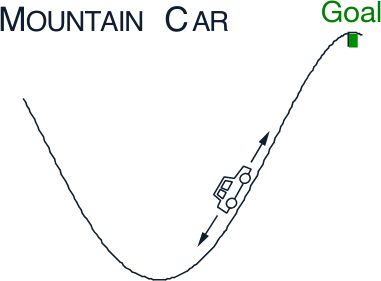
\includegraphics[scale=0.5]{img/mountainCar.png}
  \caption{Diagram of the Mountain Car environment \parencite[Figure 10.1,p 199]{Sutton18}}
  \label{fig:mountainCar}
\end{figure}

Mountain Car \textbf{(MC)} is a control problem in which a car is placed on a track in a valley between two mountains as shown in Fig. \ref{fig:mountainCar}. The goal is to reach the top of the taller mountain in as few timesteps as possible. However, the car does not have enough power to reach the top of the taller mountain and so must go up the other mountain to gain the momentum needed to reach the top if the taller mountain and reach the goal position. An axiom to think of this is that the most efficient solution would be to accelerate away from the taller mountain and then continue to accelerate in the direction of movement. Once the car loses all its momentum going up the opposite mountain it will begin to go down the mountain, and if it accelerates in the direction of movement the acceleration of the cart by its own power and gravity before it reaches the bottom will give it enough momentum to reach the goal position as quickly as possible. This would be the more ‘general control problem’ as it relies on the overall selected action as opposed to each action being critical individually to the solution of the task.

\begin{figure}[!h]
  \centering
  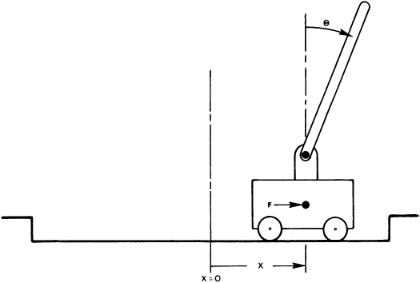
\includegraphics[scale=0.5]{img/cartPole.png}
  \caption{Diagram of Cart Pole environment \parencite[Fig. 1,p 838]{Barto83}}
  \label{fig:cartPole}
\end{figure}

The other selected control problem is Cart Pole \textbf{(CP)} which consists of a flat track on which a cart sits, this cart has attached to its center a pole mounted on a pivot shown in Figure \ref{fig:cartPole}. The goal of this task is to keep the pole and the cart within a certain range by moving the cart back and forth. This action of moving the cart allows the pole to be balanced against the force of gravity. The cart must also remain within the bounds of the track, so the goal can be described as balancing a vertical pole being pulled down by the force of gravity upon a cart, the pole cannot move beyond a range of angles centered around the vertical and the cart cannot leave a range of distances centered on the center of the track by moving the cart back and forth to correct the angle of the pole. The reward given is +1 per timestep meaning that the agent is encouraged to continue to balance the pole for as long as possible. A reward of 0 is given when the pole or the cart leaves the range, terminating the episode. This means that the CP environment is more action critical than MC as it is only when a small series of incorrect actions is taken, that the negative reward is given.
\subsection{Report Structure}
\label{subsec:intReportStructure}
This report has been composed in the IEEE Journal format with Harvard Referencing to comply with the Lincoln School of Computer Science submission guidelines. The document has been produced with intractable references allowing for section identifiers, hyperlinks and citations to link to the relevant sections in the document and web pages where applicable. For citations the year is the interactable element. Some but not all of the citations in the references section link directly to the cited literature where applicable, with DOIs and URLs. Finally in the table of contents below, the section headings link to the relevant section within this document, this can be done by \textit{clicking} on the relevant text and will be highlighted when \textit{moused over}.

\tableofcontents{}

\section{Literature Review}
\label{sec:literature}
Here the literature for each of the research requirements will be described and reviewed with attention being drawn to disparities between the literature as well as the methodological differences. This will not be a complete list of all literature cited in this report, but it will give an outline on the academic grounds of this study.
\subsection{Academic Basis}
\label{subsec:lrAcademicBasis}
The standard RL model consists of an agent interacting with an environment via perception and action. At each step of the training process the agent receives some state information. Based on this information the agent will then take an action based on it's observations of the environment. Depending on the action taken a scalar reinforcement signal is sent to the agent as a reflection of success. The agent aims to maximise the long-run sum of the reinforcement signal. This process leads to the agent choosing the rewarded actions leading to the development of the desired behaviour in the agent, as outlined in \textcite{Kaelbling96}, a survey of the RL field from 1996. This basic outline is corroborated by \textcite{Busoniu08}, a survey of multiagent RL and \textcite{Kober13}, a survey of RL in robotics. This basic conception of RL models is consistent across all literature and appears in papers up to the current day.

This learning method does not fit neatly into the two main machine learning paradigms of supervised and unsupervised learning. Instead of being directly trained by correct examples or inferring patterns from a large body of data, an RL agent learns from it's own interactions with the environment quantified by a scalar reward described in the book \textit{Reinforcement Learning: An Introduction} \textcite{Sutton18}, cited in many RL works \parencite{Amato10, Barto03, Bellemare12, Busoniu08, Gaskett99, Kober13, Smart02}. This agent driven learning style leads to a trade-off between exploration and exploitation \parencite{Sutton18, Kaelbling96, Busoniu08, Kober13}. Due to the need for the agent to explore the environment as well as perform actions to maximise the positive reward (exploitation). The trade-off stems from the incompatibility of these two behaviours which are both required for an effective agent, since the agent must explore the environment to understand the positive and negative options possible+, yet also avoid negative actions to succeed \parencite{Kaelbling96}. For most RL problems MDPs are applied as the methodology for modelling decisions to calculate action rewards accounting for the exploration-exploitation trade-off \parencite{Kober13}. MDPs work by considering rewards temporally, meaning that a series of actions can be attributed to the delayed reward function (\textcite{Kaelbling96, Busoniu08, Kober13}). This is in contrast to more simple greedy strategies which reward the agent directly for each individual action. However these methods can fall victim to unlucky reward sampling early in the training process (\textcite{Kaelbling96}). A useful framing problem for understanding the balancing of exploration and exploitation is the K-Armed Bandit problem. This is used in most survey papers (\textcite{Kaelbling96, Busoniu08, Kober13}) to explore the performance of RL methods in the scope of exploration vs exploitation. The more recent papers \textcite{Busoniu08, Kober13} analysing these methods to balance exploration and exploitation tend towards the more dynamic methods like MDPs as opposed to the more simplistic greedy strategies mentioned in \textcite{Kaelbling96}. The other simplistic methods suggested by \textcite{Kaelbling96} are not mentioned in the more recent surveys of RL \textcite{Busoniu08, Kober13}, only in \textcite{Sutton18} are these methods mentioned as introductory methods to RL. The literature seems to be in agreement on many of the details of RL methods, however many methods mentioned in the older \textcite{Kaelbling96} seem to be less widely discussed in the surveys written in recent years \parencite{Busoniu08, Kober13}. This may be suggestive of advancements in RL methods making these older methods obsolete or irrelevant which is interesting in such an empirically research based field as ML.

Most of the methods discussed in RL are very old, for example MDPs were originally proposed by \textcite{Bellman58} in 1958 which is cited in each of the RL surveys \textcite{Kaelbling96, Busoniu08, Kober13} as well as the seminal \textcite{Sutton18}. The vast majority of improvements made to RL methods are minor improvements to MDPs.
\subsection{Scope of Reinforcement Learning}
\label{subsec:lrScope}
Reinforcement learning (RL) is a very adaptable machine learning method due to the wide range of approaches and methodologies that can be used to form a solution. However \textcite{Kaelbling96} concludes that RL performs well on small problems but poorly on larger problems due to its efficiency of generalising the problems. This point is reaffirmed by \textcite{Wirth17}, adding that an efficient generalisation of a complex problem requires expert domain knowledge. This suggests that whilst versatile, RL is only generally suited to simple or well defined problems.

One of the primary areas of RL research is robotics since the domain of controlling a robot fits neatly into an RL problem as discussed in \textcite{Kober13}, whereas other machine learning disciplines are very difficult to utilise for robotic control systems. This view of RL in robotics is shared by \textcite{Smart02}. Many other hurdles are introduced by using reinforcement learning in a real context such as observation inaccuracies and the expense of hardware \parencite{Kober13}, however this does not pertain to this project. Robotic RL agents instead present a strong base of real agent-environment interactions \parencite{Kober13}.

Up until this point only single-agent systems have been discussed, however Multi-Agent Reinforcement Learning \textbf{(MARL)} is another large body of work with multiple agents training in the same environment. In ways this domain is similar to single-agent RL, but multiple agents open up a new set of challenges and advantages to the learning process. As described in \textcite{Busoniu08} the main challenge faced is an exacerbation of the exploration-exploitation trade-off due to inter-agent interactions adding a new level of complexity to the issue. Multiple agents can also be turned into an advantage in MARL by allowing agents to share their experience with other agents, making the learning process more data efficient as a result. Additionally more advanced reward functions can encourage collaborative actions between agents. One clear advantage of MARL over other RL domains is the opportunity to  benefit from parallel computing which increases computational efficiency.

Most RL environments could be described as games; unsurprisingly the most active domain of RL is playing video games. Video games present a host of environments easily adaptable to RL applications, however the low complexity tolerance of RL still takes effect. This leads to either very simplistic games being used to train complete agents to perform well such as in \textcite{Bellemare12} or more high level applications like \textcite{Amato10} where an RL agent controls the strategies of an artificial intelligence agent designed to play the game. These applications both use MDPs with QL to consider the higher level strategy required for playing video games.

A criticism is raised in \textcite{Shoham03}, a critical survey of MARL using MDPs, as to the definition of many RL solutions in that they are often performed from an ill defined domain basis in how learning best occurs. It outlines a four stage method of properly defining an RL problem, describing how too many RL solutions work off previous bases without exploring their applicability to the problem being addressed. This is demonstrated by the contrast between \textcite{Amato10} where little academically supported domain knowledge is presented versus \textcite{Ng06} where the domain knowledge is comprehensively explored before designing the RL solution. This suggests that certain areas of RL problems are ill guided. This should remain pertinent through this research project and be addressed where applicable. 

\subsection{Reinforcement Learning Techniques}
\label{subsec:lrRl}
Whilst not encompassing all of RL, MDPs represent the vast majority of reinforcement learning solutions. This is due to the simplicity with which a complex problem can be represented, taking into account time and previous actions as outlined in \textcite{Barto03}. As a result of this focus there is a wealth of different MDP strategies in the literature to draw from. An MDP is a framework for modelling actions with controllable yet undetermined outcomes to be optimised \parencite{Bellman58}. Utilising an MDP a complex problem can be abstracted down to a comparably computationally simple problem. This however requires much domain specific knowledge to be properly exercised \textcite{Shoham03}.

Markov Decision Processes (MDPs) are a mathematical framework to quantify and rationalise decisions made in a Stochastic Game (SG) \parencite{Bellman58}. SGs are step by step games which quantify an environment probabilistically \parencite{Shapley53}. This hugely simplifies reward and action computation in RL problems \parencite{Busoniu08}.

In both \textcite{Bellemare12, Amato10} QL is used. It is an approach to MDPs which allows an RL agent to explore an environment to experience the various reward states associated with each action. The QL task will use these immediate rewards to plan temporally how to maximise the reward overall as described in \textcite{Watkins92}.

Double Q-Learning (DQL) is an optimisation of QL to reduce the overestimation bias seen in QL. This overestimation is a result of having more encounters with a certain state action pair. A concise example of this can be found in \textcite[p. 110]{Sutton18}, where a simple control problem is solved using both QL and DQL. The control problem presents more options in one direction than the other, despite the direction with one path giving the best reward. On this control problem QL routinely spends more episodes performing the un-optimal actions as a result of overestimation leading to maximisation bias. Whereas DQL very quickly converges towards the optimal policy when compared with the results for QL, and converges much closer to that optimal policy. This is also discussed in \textcite{Hasselt10}, the paper to first propose DQL. The mechanics of DQL are very similar to QL except, instead of using a single Q-table, two Q-tables are used in conjunction but are updated in an isolated fashion so that the two tables are trained on individual samples of the environment data. However since both tables are used to select the optimal action it is no less data-efficient. As a result maximisation bias is minimised leading to more robust policies over QL at the expense of a slight underestimation bias.

There are a myriad of other QL-like methods including Expected SARSA analysed in \textcite{Seijen09} which performs QL with a traditional off-policy method except that it factors in what the more likely action selection is when deciding on the action to assess. Making it similar to an on-policy control method. Another would be Backward Q-learning outlined in \textcite{Wang13} where both control policies are used in conjunction to first learn the policy using an off-policy control method and then revise that policy using an on-policy control method. Others include Deep Q-Learning in \textcite{Hausknecht15} where a Recurrent Neural-Network is used to perform value approximation for a Q-table. Another interesting example related to this study would be Deep Double Q-Learning proposed by \textcite{Hasselt16} which is similar to DQL but applied to a Deep Q-Learning method. But since this is to be a direct comparison between the control methods only QL and DQL, however their Deep Learning counterparts in \textcite{Hausknecht15} and \textcite{Hasselt16} respectively. These provide an interesting step for future research on this topic as it would allow for more advanced learning environments to be used in comparison such as the Atari 2600 library as in \textcite{Mnih13} which would provide far more grounds for potential analysis.

Much of the research pertaining to RL problems seems much too condensed, with single authors appearing in multiple papers such as Barto in \textcite{Barto03} as well as the book \textcite{Sutton18}. Kaelbling also appears in both \textcite{Kaelbling96, Smart02}. Other concentrations like this appear all across the RL literature which makes me sceptical of the academic basis of many of these methodologies.
\subsection{Validation Methods}
\label{subsec:lrValidation}
Validation methods for RL solutions vary wildly since each application has a differing goal state. Unlike supervised and unsupervised learning, success of an RL agent is entirely subject to the task at hand \parencite{Kaelbling96, Busoniu08, Kober13}. A broader search of specific RL applications will be required to effectively devise a methodology for validation of RL implementations, although it is highlighted in \textcite{Shoham03} that domain specific knowledge should be used to devise a testing methodology.

To circumvent this issue, common control problems will be used from the academic literature so that methodologies and results can be meaningfully compared. One example of a ubiquitous control problem is Cart Pole (CP), originally codified in an RL context by \textcite{Barto83} and refined to a TD context by \textcite{Moore90}. This control problem is used in \textcite{Nagendra18}, \textcite{Wang13} and \textcite{Seijen09} to compare the performance of model-free RL methods, although there is no standard of implementation among these studies. Another common control problem used is Mountain Car (MC), which unlike CP is often used as a benchmark for new RL methods as opposed to comparative analyses. MC is used in \textcite{Waldock08} and \textcite{Wang13} to compare TD control algorithms. These uses of MC are much more consistent than that of CP in academic literature.

In the RL literature there is very little in common between the analyses used for comparing Rl agents, the only ubiquitous metric compared between the previously mentioned studies is average reward. This does however make sense as this is the most obvious and representative metric that can be measured as a reflection of an agent’s performance. However, there is much variance in agent performance and so the average reward is primarily used. This can hide aspects of the agent performance and within the literature there is very little discussion of this. The other common method of comparison is mapping of the actions taken, this is done to great effect in \textcite{Corozza15}, a study of Q-Learning and SARSA in the context of financial trading. But this is done very poorly in \textcite{Nagendra18}, where the plots are near incomprehensible, although this could be an effect of compression for the version read. This would appear to support the findings of \textcite{Shoham03} that analysis of an RL agent is very dependent on the task it is completing. Consequently in the case of this project the reward will likely be the only metric that can be reliably compared.
\subsection{Project Management}
\label{subsec:lrProjMan}
There is little academic writing on project management methodologies specifically for machine learning projects, but this is understandable as it has only recently gained large scale adoption in professional applications. Additionally, there is very little discussion in most papers analysing QL on the specifics of their implementation. This led to the search for a methodology with informality in the design process which could be adapted to changing requirements. As the research on the theory of QL informed the design of the artefact and in turn the requirements of the project management methodologies. The rise in popularity of Agile methodologies appeared to be the most appropriate place to \textit{‘dive in’}.

Agile software development was first inspired by the ‘Manifesto for Agile Software Development’ \textcite{Beck01} which was signed and supported by many eminent people in the software development industry at the time. This began a shift away from the top down project management methodologies in the software industry into Scrum and Extreme Programming as described by \textcite{Matharu15}, an empirical study of Agile software development. This comparative analysis compares the three most popular Agile methodologies of Scrum, Extreme Programming and Kanban and discusses their adoption among software development firms. In particular, Table 2 in \textcite[p. 4]{Matharu15} directly compares each methodology’s approach to specific parameters. This table in particular was very beneficial to the further research of software development.

\textcite{Ahmad17} is a systematic mapping study of Kanban in software engineering. This paper is an extension of a 2013 literature review by the same author. \textcite{Ahmad17} combines a survey of the academic literature with experience reports from Kanban implementations in the industry. It reports on the benefits and challenges identified in Kanban applications and recommends best practices for implementation of a Kanban methodology. Interestingly, many of the findings of this paper contradict the findings previously discussed, although the main focus of \textcite{Ahmad17} was on implementation in mature industries and indeed the challenges identified corroborate this: It was mainly difficulty in the transition process and not with the functionality of Kanban. An experimental application of Kanban principles by \textcite{Mahnic13}, compared with a previous experimental application of Scrum in 2012 by the same author, supports this; as by slowly incorporating Kanban principles into an existing methodology like Scrum makes this transition much easier for the team members. Then encouraging the team members to adapt the Kanban process to suit their workflow. This contrasts \textcite{Ahmad17} by reporting that users of the process should experiment with and adapt the Kanban process to their environment, whereas Ahmad states that the Kanban process should not be changed without approval of upper management and the stakeholders. This is perhaps the most obvious example of how Kanban works best when implemented organically, allowing the users to grasp the process and adapt it to their specific needs \parencite{Mahnic13}.

One particular Agile software management methodology gaining traction is Lean \parencite{Corona13} which, similar to the Agile manifesto by \textcite{Beck01} prescribes a mindset of developer focused management. This is described in \textcite{Poppendieck13} as devolving responsibility to the team working on the project, instead of having external management dictate the process. Encouraging team members to take organisational matters into their own hands allows them to adapt the processes to fit their needs. As opposed to Agile, Lean is less of a complete methodological family and more a toolbox of prescriptions to augment Agile to specific use cases \parencite{Corona13}. However, Lean is more focused on industrial applications, and so these prescriptions must be taken piece-meal and incorporated into the methodology in order to be used for this project. In \textcite{Corona13}, Kanban is described as the most popular and effective tool to bring Lean principles into a more cohesive project management methodology.
\subsection{Open-Source Software}
\label{subsec:lrOss}
Open-Source has become increasingly used in the software industry; what was once considered inferior ‘free software’ has rapidly matured into a myriad of mature ecosystems \parencite{Morgan07}. This change has also coincided with a new movement, particularly in research, towards sharing of developed knowledge \parencite{Sauer07}. This has been particularly impactful in Data Science and Machine Learning where the open access to large datasets has been revolutionary.

In \textcite{Sauer07} and \textcite{Morgan07} the non-pecuniary benefits of Open-Source Software \textbf{(OSS)} are discussed. The academic understanding of OSS is called into question in \textcite{Sauer07} in which a new model for understanding the benefits is proposed. This model lacks sufficient data to be put into practice, but in the examples recorded by both \textcite{Sauer07} and \textcite{Morgan07} such as the Linux operating system, huge advantages are seen. These advantages listed in \textcite{Morgan07} include: reliability, quality, performance and flexibility. This would make sense as the software is developed by the users and so in terms of methodology these would be the stake-holders. Whilst OSS lacks certain qualities like dedicated user support, its benefits specifically for researchers and software developers are undeniable \textcite{Sauer07}.

The research into the phenomenon of OSS is sparse but agreement on the benefits is ubiquitous, the only shortcoming of the literature is that like much of the software development literature, industrial application remains the focus. Some incredible examples of OSS being created are Scipy\footnote{Scipy: \url{https://scipy.org/}} which has revolutionised scientific computing.

\section{Methodology}
\label{sec:methodology}
The aims of this project are to perform an empirical comparison between the Q-learning and SARSA control methods across reinforcement learning environments. There is a distinct lack of any academic work directly comparing the control methods without being aimed towards Deep RL, with on-policy and off-policy most often being a side note in the grander analysis being done such as \textcite{Nagendra18}; or in the case of \textcite{Corozza15} the environments the control policies are being tested in are highly specialised. The information needed to perform this analysis is well documented and has been for years, but there is a noticeable lack any direct comparisons between the differences of the two control methods. In this analysis the aim is to draw the most simple and direct quantitative comparison possible between these two, as well as describe the process of how they function, as another missing part in the literature is a concrete example of how the methods should be implemented and the difference between them in practice. The focus of the artefact will not only be to perform this direct analysis, but to give a concrete example of these control policies and present a basis for future development into other problems. To achieve this, an iterative, test-driven development process, drawing from a robust theoretical outline should be used.  The development experience from this process will present a comprehensive analysis of the methods utilised by basic Q-learning, translating them into practice with explanation of how individual elements work as well as how they interoperate as a complete machine learning solution. This will be accompanied by an explanation of the theoretical ideas that describe the process mathematically and conceptually.
\subsection{Project Management}
\label{subsec:mthdProjMan}
This project is to be developed independently and so the majority of academic writing on project management approaches will not apply directly. However certain aspects can be used to formalise an independent design and development process and so here these will be discussed. The primary focus of this is organisational structure, integrating the design, development and testing phases. Much of the literature on project management methodologies focuses on this specifically. However the primary focus is usually having separate teams working on this process collectively.

In the case of this project there is little need for this collaborative focus and so the main basis for the project management methodology design will be on Kanban. This is due to its focus on visualising and limiting the amount of work-in progress during development \parencite[3]{Matharu15}. This is opposed to other Agile methodologies where the design principles involve comprehensive planning of what is to be developed and how. This would not fit this project as the aim is to design and build small parts of the problem at a time to allow for comprehensive testing and understanding of each component as it is added. Using the notes and record of the tasks on the Kanban board would be helpful in developing a complete picture after the fact to allow for a well informed and comprehensive analysis of the resulting RL agents and surrounding research.

Kanban has its roots in the manufacturing industry but has been adapted to many different fields. In \textcite{Matharu15} this adaptability is ascribed to the simplicity of the methodology. By streamlining workflow and presenting tasks visually the project, as a whole, becomes easily interpretable by any team member \parencite{Ahmad17}. This is helped by the interdisciplinary team structure of Kanban comprising multiple specialists in the project domain \parencite{Matharu15}. Whilst these aspects do not directly apply to the independent nature of this project the team ownership aspects apply very strongly. This also speaks to the compatibility of Kanban with many different project domains. This is useful to this project as there are not only software development processes, but also research and analysis processes. Each of these processes can be optimised organisationally with the Kanban project management methodology.

Yet another strength of Kanban for machine learning projects is that unlike Scrum with no formal testing approach and Extreme Programming with strongly test driven development \parencite{Matharu15}, Kanban uses a pull and push process to define entry and exit criteria from each stage in the process \parencite{Ahmad17}. This means that whilst the development isn’t directly test driven it instead provides framework to apply strong testing criteria to each work product. But additionally this can be changed on a project-to-project basis, for example a review step could be one of the exit criteria for the research method and indexing of results on the statistical analysis Kanban processes.

The informal nature of Kanban also makes it very adaptable to change, with no formal structure to the process other than the Kanban board and the limiting of workflow \parencite{Mahnic13}. This also means that the team can adapt the process at any time, for example changing the limit on work-in-progress items or adding new items, even adding a column for work items which need to be paused until other items it depends on are completed \textcite{Ahmad17}. Since the nature of the project will adapt as a stronger understanding is built, this is very suitable.

Another use for Kanban will be in organisation of report production, for example after completing a section it could be moved to a review section. Then, finally, it can be moved to a draft section to be reviewed  by peers, before document production. Another use would be adding citations to the bibliography in a batch after section completion as an exit criteria of the writing process section.

Overall Kanban seems to be a very useful tool in planning and executing the various elements of this project and will be employed universally for all individual elements as well as managing overall flow such as pausing software development to perform more research in a new area highlighted by the experience in developing QL agents.
\subsection{Software Development}
\label{subsec:mthdSoftDev}
The particular strength of Kanban in software development comes from the team owned and driven process \parencite{Matharu15}. This allows for a conceptual model of the final product to be formalised by the team to focus the workflow in the areas needed \parencite{Matharu15}. In particular, all elements of the process are to be kept available for all team members at all times to make alterations and discuss the process \parencite{Mahnic13}. In the software development industry Kanban is often synthesized with other Agile methodologies to suit the particular use case \parencite{Ahmad17}. This resilience of Kanban to changes in the process makes it highly adaptable to any use case in Agile software development methodologies. The entry and exit criteria also make for a tightly controlled development cycle, but without the need for extensive planning of the process increasing lead-time \parencite{Ahmad17}. This suits a more emergent nature of task addition, since as the software is developed, more experience with QL will allow for optimisations and additions that would not have been realised at the beginning of the process.

Since the development of the RL agents before any experimental analysis can be performed is so holistic in nature, it would make little sense to separate the workflow any further than the discrete elements to be added. For this reason the short iterations of Kanban make the most sense. Since the project workflow will be done on a piece-by-piece basis, it would also not make sense to consider the more top down methodologies like Waterfall which the Agile methodologies were designed to replace. One of the primary design factors behind the Agile was adaptability to changing customer requirements \parencite{Beck01}, but this is not so pertinent to this project. The less customer focused approach is yet another strength Kanban has over the other Agile methodologies; as the focus is entirely on the team to organise the project to fit requirements based on their understanding of the project and the cumstomer requirements \parencite{Ahmad17}.

Some particularly pertinent examples of benefits to the process in relation to this project include: ‘Better control of project activities and tasks’, ‘Identify impediments to flow’ and ‘Improve prioritisation of products and tasks’. Combining this with certain Lean principles would streamline the development process massively. Additional benefits to the organisation and team members are: ‘Improve team motivation’ and ‘Promoting a culture of continuous learning’ \parencite[Table 13,105]{Ahmad17}. These benefits would be very impactful on this project as it is being undertaken in a studious manor, especially since as an individual project the need for motivation and learning during the development process is likely to be a primary factor in the development process.

The synthesis of Lean principles into Kanban processes has seen accelerating adoption in the software industry. It would appear that the two approaches are very compatible as instead of focusing on process design they both focus on emergent process efficiency \parencite{Ahmad17}. For this reason Lean principles will be incorporated into the software development methodology to augment Kanban to better fit the particular needs of this project. Selected from \textcite{Poppendieck13}, these Lean tools will augment the Kanban process to be more suited for this project. The first is ‘Increase Flow’ by focusing on keeping the implementation simplistic. The entire process will flow better as a result and be much more adaptable for refactoring as the complexity develops. In particular the focus will not be on computational performance but on usability and adaptability to different problems. Another Lean principle is ‘Keep Getting Better’ which focuses on applying discrete analysis of the project using the scientific method to implement the best version of each iteration of experimentation. Finally ‘Enhance Learning’ which augments the usual project management approach of planning with the more adaptable and emergent process of learning. This helps by trusting the people working on the project to make the right call and not discourage retroactive changes based on their developing knowledge of the project and it’s requirements. Implementing these principles into the Kanban process should allow for a productive and well organised software development process.

As discussed in Section \ref{subsec:lrProjMan}, \textcite{Corona13} points to this devolved and flexible project management methodology for software development being very powerful in revolutionising how small teams operate. Additionally, unlike Agile and Scrum where the use of tools was discouraged in favour of face-to-face interaction and physical displays of project flow, Kanban instead encourages the use of tools for the implementation of the Kanban board \parencite{Corona13}. This has made it particularly popular with distributed teams, with the rise of tools like Trello\footnote{Trello: \url{https://trello.com/}}. One particular strength for this project is the ability to create multiple digital Kanban boards for different parts of the project, for example, each new branch created in software development.

Version Control Systems \textbf{(VCSs)} (also known as Source Control) are another important element of this project as a process to formalise development. VCSs work by tracking changes made to a codebase, this allows for any point in the development process to be examined. By each change made being logged with notes on why and to what effect, a rich history of the development process is created. This data on its own allows for analysis of the development process and particularly graphing of the history of changes and development progress \parencite{Ball97}. This data extraction would not be possible without consistent reports of changes made to the codebase which would be incredibly hard to implement without a system designed to facilitate it, the system being designed around these principles requires very little extra work \parencite{Spinellis05}. In the context of Kanban, VCSs augment the development process further by allowing each work item to be tracked through development. Additionally, the discrete nature of work items compliments the atomic change style of VCSs. For example if one work item is a change to happen in multiple places and files within the same codebase, these can be recorded in the version history as one change. Within this change multiple edits will be listed to all the files changed \parencite{Spinellis05}, by recording this as part of the exit criteria for a column on the Kanban board a comprehensive picture of the development process can be created. The main application of VCSs is to allow for effective development of one codebase by multiple developers, which is not terribly pertinent to this project, however the ability to maintain one cohesive version across multiple devices is. Particularly for this project the need to use all of the computational power available on one device for testing requires a second device for development so as not to hamper either process by the computational needs of the other. However, changes will need to be made to the same codebase on both machines as the testing may require a need to adapt some parts of the codebase, for example when errors have been encountered. By making the change on the testing device, time is saved in the process of corroborating the change between devices. But VCSs allow for changes to be made on both devices independently and then merged together once testing is complete \parencite{De-Alwis09}.
\subsection{Toolsets and Machine Environments}
\label{subsec:mthdTools}
The aim of this project is to develop and test on-policy and off-policy control methods for traditional control problems using Q-Learning. The developed artefact should be a clear example of how Q-Learning should be implemented and demonstrate how the control methods could be expanded to different problems. Developed as an Open-Source demonstration, it should be easily accessible and virtually portable to allow others to learn how to implement and use this style of RL. The implementation should be simple to allow for fast iteration and easy adaptation, this simplicity will also considerably aid in the addition of optimisations once the agent has been developed. A testing infrastructure should also be added to allow for long-run experiments to be run, testing  multiple parameters at once. 

Continuing on from the discussion of OSS in Section \ref{subsec:lrOss}, the machine learning software ecosystem is particularly rich with examples of successful OSS. In particular TensorFlow\footnote{TensorFlow: \url{https://www.tensorflow.org/}} which is a framework for building machine learning models with arbitrary parallelisation, allowing for GPU acceleration. Scikit-Learn\footnote{scikit-learn: \url{https://scikit-learn.org}} is a library built upon the Scipy family specifically for data analysis which has seen widespread adoption by the machine learning community. The ability to study and change source code is essential in scientific computing specifically, and this makes machine learning a natural fit to the Open-Source model. Following on from this, the project is to be OSS and so will need to be distributed and source controlled. The premier version control software (VCS) is Git, in the 2018 StackOverflow developer survey\footnote{StackOverflow developer survey: \url{https://insights.stackoverflow.com/survey/2018\#work-_-version-control}} it is used by 87.2\% of respondents. Git is also OSS and was originally developed for use by the Linux maintainers, source control keeps track of changes made to files it records and keeps a complete history of their development. Git is primarily used to share code among multiple developers although it is particularly useful in this project in that it can be used to maintain one version across multiple devices. The most widely used hosting platform for Git usage and the largest host of source code in the world is GitHub \parencite{Gousios14}. GitHub not only functions as a hosting platform for Git source control but also includes a range of features, making it particularly useful for open source development. One particularly interesting feature is the ability to create virtual Kanban boards which is how this Kanban implementation will be managed in this project.

Git will be particularly useful in this project for facilitating the separation of the main stable trunk from development branches \parencite{De-Alwis09}. By doing so the possibility of breaking unexpected parts of the code is eliminated on a system wide scale. Instead a development item can be developed and tested separately from the main codebase, finally being added to the main codebase once development and testing are complete. These branching mechanics are a key feature of Decentralised VCSs, of which Git is the most widely used \parencite{De-Alwis09}. This means that even if multiple items are being developed simultaneously they cannot interfere with one another and the last working version is protected from changes made in either branch. Git provides a simple interface for merging these branches back into the main trunk upon completion which facilitates a complete review of the changes made in the development branch against the main trunk. Git also provides an interface for maintaining one version across multiple devices with the merge allowing for these changes to be compared and selectively added to the main trunk. Particularly in this project the computational requirements of RL dictate a need for multiple machines for efficient development and so it is imperative that a VCS be used and of these Git contains the most features to directly support this need.

Machine learning in particular has a strong dependency on libraries for numerical computation, specifically array manipulation. This rules out the more scientific languages like Matlab and R as their library ecosystems are not as featureful as more widely used languages such as C++, C\# and Python. These each have their own problems though as C++ is by far the most runtime performant language available for machine learning, but suffers from needing to compile before execution and a very strict syntactical style. C\# is similar to C++ in that it is performant at runtime but benefits from much wider use in the machine learning community meaning it has access to far more libraries than C++ specifically built for machine learning use cases. C\# also has a far more succinct syntactical style meaning it can do much the same as C++ but considerably more compactly. This is useful for decreasing iteration time and allowing review of the code. However C\# also suffers from needing to compile before execution. This issue of compilation is not an issue for deployment applications but in a test-driven process like this project, the compilation times would add up to a considerable time loss. Python on the other hand is interpreted at runtime, in this sense it is more a scripting language and so suffers in runtime performance quite dramatically when compared to the C family of languages. However Python is a high level language unlike C++ and C\# and so benefits from an incredibly simplified syntax style. This makes Python code considerably more condensed and also greatly improves readability. In an empirical study \textcite{Prechelt00}, this condensed and readable syntax has been shown to increase productivity over C++ by half. Python also benefits from being a scientific language and so comes with many useful features built in such as the ‘math’ library for doing advanced calculations like exponents. Finally the libraries available for Python are truly staggering, PyPI\footnote{Python Package Index: \url{https://pypi.org/}} reports over two hundred thousand packages available. One library in particular has been seminal in machine learning development, that being Numpy\footnote{Numpy: \url{https://numpy.org/}}, written in lower level languages like C, C++ and Fortran it takes advantage of their runtime performance and allows for efficient manipulation of arrays of any size. This is particularly pertinent to this project as a Q-table is only an array, and so the ability to manage this array efficiently is essential.

The library to be used is OpenAI Gym\footnote{OpenAI Gym: \url{https://gym.openai.com/}}created by OpenAI, a large center for reinforcement learning research. In the whitepaper accompanying the launch of Gym \textcite{Brockman16} it is described as so: “OpenAI Gym is a toolkit for reinforcement learning research.  It includes a growing collection of benchmark problems that expose a common interface, and a website where people can share their results and compare the performance of algorithms.” This framework offers both a myriad of reinforcement learning environments to experiment with but is also OSS and so the source is freely available for study. This is exceptionally helpful for RL applications since an understanding of the environment is a prerequisite to effective implementation of an agent.

Since there is no intended use-case for this project the focus will be on simplicity. To allow the project to be used anytime, anywhere, by anyone. This means that there can be no environmentally dependent factors, because of this  there will need to be dependency control as well as source control. This will keep track of the packages used and allow them to be installed in a virtual environment. To achieve this portability, the pipenv\footnote{PyPI Database (pipenv): \url{https://pypi.org/project/pipenv/}} module for pip\footnote{PyPI Database (pip): \url{https://pypi.org/project/pip/}} will be used, the package manager for the PyPI Database\footnote{PyPI Database: \url{https://pypi.org/}}. Allowing for the requirements of a Python project to be frozen and installed by a user into a separate, virtual, working environment with the pipenv tool. The virtualization of this environment avoids dependency clashsd and versioning issues when integrating with the user’s current Python environment.
\subsection{Statistical Analysis}
\label{subsec:mthdStats}
In this project the aim is to compare the performance of QL agents against one another. As discussed in Section \ref{subsec:lrValidation} there is one ubiquitous metric to do this by, that being the cumulative reward obtained in each episode. In CP this reward is positive and so the aim is to keep performing the task for as long as possible, whereas in MC the reward is negative meaning the aim is to complete the task as fast as possible. Since the reward is constant with time there is little more to be gleaned from it than that and so instead the statistical distribution should be analysed. This will include measurements such as the: average, mean, maximum, minimum, upper and lower quartiles. Additionally the standard deviation would be a useful metric to compute from the concentration of rewards. There are two phases in which this data can be recorded the first being testing where the agent’s policy is tested directly once the learning has completed. Also the performance can be tracked during the learning process, this comes with challenges however since the learning process can vary wildly. Indeed as can the tested results. For this reason a certain degree of sampling will be required to get statistically stable results using averages. For example the overall learning and testing phases would be repeated a number of times and the performance reported as an average of these results. However this would also retract from the statistical accuracy of these results to the actual results. As a measure of this however, standard deviation would be used to give a numerical score of the variance of these results. These combined give both a measure of overall performance as well as the stability of that performance which would answer the hypothesis posed in Section \ref{subsec:intHypothesis}.

The results will also be plotted so as to allow for more direct analysis and comparison of the results. In particular the best representation of the performance distribution as the result of multiple runs of an experiment would be a notched box plot. A notched box plot represents the data with a line at the median extending a box to the upper and lower quartile, with a notch around the median denoting the confidence interval of the median. This box is then extended by whiskers to either the maximum and minimum of the distribution or $\frac{3}{2}$ times the interquartile range. With data points in the distribution being plotted as dots if they fall beyond the whiskers. This gives a very simple representation of a statistical distribution and conveys both the internal distribution of that data as well as any outliers. The recorded averages will then also be plotted in a line graph atop the box plots to give a representation of fluctuation between the experiments. Another useful plot for understanding the learning process of an agent is an averaged line graph of the measurement of reward per episode. To further normalise this data the distribution could be recorded into bins of a certain length to allow for yet more stability in the plotting the learning performance.
\subsection{Research Methods}
\label{subsec:mthdRes}
As this is an empirical comparative analysis it is not surprising that primarily quantitative experimental research is to be done. There is however an element of qualitative research in that the empirical findings will inform the analysis of the academic literature as per the hypotheses Section \ref{subsec:intHypothesis}. Indeed the majority of the studies cited in this report use primarily quantitative, experimental research methods. The research methods used in the more explorative studies such as \textcite{Wang13, Waldock08} are very similar to those used in the comparative studies such as \textcite{Corozza15, Nagendra18, Seijen09}. Both styles of paper demonstrate their results using plots and tables of their findings. Usually these are of reward results although many of the problem domains for example \textcite{Corozza15} includes presentation of actions taken over time. But the bulk of traditional RL research follows a similar research methodology of presenting experimental results. This project will follow a similar methodology of experimental evaluation and presentation of results before using the findings to compare against other similar results in the literature before reflecting on the literature as a whole to answer the research questions posed Section \ref{subsec:intAimAndObj}.
\section{Design and Development}
\label{sec:design}
In this section, the process of developing and testing the reinforcement learning agents will be discussed. Expansions of the ideas presented in the introduction Section \ref{sec:introduction} and literature review Section \ref{sec:literature} will be included and reference their previous inclusions where appropriate.

The design of the artifact will be addressed in a chronological fashion to outline the learning process through the development of the QL agents using OpenAI’s Gym library as outlined in Section \ref{subsec:intAimAndObj}. This should function as an implementation guide for generic QL agents since the academic literature lacks such an example.

The source code for the developed artefact as discussed in the report is available on GitHub\footnote{GitHub - Q-Learnin (tagged report version): \url{https://github.com/podit/Q-learnin/tree/report}}, links to each script will be given when they are being discussed alongside code snippets and in Appendix \ref{apx:sourceCode}. Development will continue after this dissertation and can be found on GitHub\footnote{GitHub - Q-Learnin: \url{https://github.com/podit/Q-learnin}}.
\subsection{Requirements Analysis}
\label{subsec:desReq}
The analysis of the requirements for this project was very important, as with machine learning the functionality of the work produced is not the goal - the overall performance is. Whilst an agent can be capable of performing the task, it is only by analysis of the results that it can be said to be working correctly. This means that experimental analysis is par for the course when developing any machine learning project. Therefore, a complete picture of the task must be developed early-on to allow for effective development of the project. In this section the theoretical background will be presented for the project as well as analysis of the hardware and software requirements needed to perform it.
\subsubsection{Requirements}
\label{subsubsec:desReqReq}
This will be a discussion of the basis of the requirements for analysis of the problem domain to inform development going forward. As well as this, it will discuss how to understand the limitations that the artefact will be developed within.

It is important to first have a clear understanding of the supporting theory so results can be clearly analysed. This will also help in decomposition of the problem for software development during the design and development stages. There is a lot of writing on RL to explain the theory behind it, but there is little in the way of presenting a unified view of how RL should be done. This means that to understand the theory, a lot of analysis of the underlying mathematics and ideas is required in order to grasp the task as a whole, so that RL can be effectively implemented in practice. The seminal piece in the understanding of TD learning is \cite[Ch. 6]{Sutton18}, which is cited in most academic work on the subject. It gives a comprehensive yet approachable description of the field, giving examples and explanations of what TD learning can be used for. The underlying mathematics of Rl is also presented in a manner that is easy to understand.

As discussed in Section \ref{subsec:mthdTools}, the RL agent is to be implemented using Python to solve the MC and CP control problems using OpenAI Gym. These tools were chosen for their syntactic simplicity as well as the resulting short iteration time. This will allow for the agents to be refactored multiple times in a simple way, which will result in a more approachable implementation and a more optimised agent. The aim for this software is not to be the best performing or fastest at solving environments using these algorithms, but to demonstrate an approachable and clear example of how they should be utilised for solving simple RL problems. It should also serve as a good basis from which to conduct the experimental analysis of on-policy and off-policy control methods.

One particular bottleneck that must be accounted for is RL’s incompatibility with any degree of parallelization. Indeed, the only way this can be achieved using traditional methods, is to have multiple agents learn simultaneously and share their experience \parencite{Kretchmar02} which would not suit this analysis of control methods as it could distort the differences between on-policy and off-policy control methods. Without moving to deep reinforcement learning, there is little way around this particular bottleneck. This means that the testing and development of the RL agents will be limited to the eight cores of an i7-2600\footnote{Intel i7-2600: \url{https://ark.intel.com/content/www/us/en/ark/products/52213/intel-core-i7-2600-processor-8m-cache-up-to-3-80-ghz.html}} and their single thread performance. Careful consideration must be given to this issue, as testing performance to statistical stability will take a lot of time and therefore, this compute time will need to be carefully managed.
\subsubsection{Design}
\label{subsubsec:devReqDes}
To understand the fundamental limitations of TD learning, a complete analysis will need to be done of the algorithms and mathematical frameworks which will make this possible. To do this,  \textcite[ch. 6]{Sutton18} will be used as a guideline for overall understanding and surrounding reading of the original papers listed in the ‘Bibliographical and Historical Remarks’ section at the end of the chapter. These will include \textcite{Bellman58} to study how the Bellman equation is exploited by TD methods in QL and how TD learning described in \textcite{Sutton87}, derived from the original MDP framework. Additionally, \textcite{Hasselt11} will be consulted when reading into detailed examples of the algorithms implemented and mathematics used in TD learning methods and their performance. Finally, this mathematical and functional understanding will be analysed through the lens of the RL methods being used, these being \textcite{Watkins89, Watkins92} for QL and \textcite{Hasselt10} for DQL.

Methods for working within the hardware bottleneck will be planned so they do not delay development progress as a result of waiting for results. Methods to reduce system load for maximum computational efficiency will be investigated to make the results needed to test the agent as fast to obtain as possible. These environmental restraints will be explored to find the optimal workflow for this development cycle.
\subsubsection{Implementation}
\label{subsubsec:desReqImp}
Most of RL is built upon optimisations of dynamic programming (DP) algorithms, which are used to compute optimal policies from a perfect model of the environment \parencite{Sutton18}. In the foundational text by \textcite{Bellman58}, the differential functions for continuous environments, typical of DP, are applied to a discrete system for “the use of digital computers”. This brings DP into the realm of stochastic sequences allowing for the application of discrete Markov Decision Processes (MDPs). In the explanation given in \textcite[ch 4,p 234]{Bellman58}, this discretisation is done in \emph{time} to allow for the comparison of one state to the next state in a stochastic fashion. It is from this that a Temporal Difference (TD) model can be constructed to optimise the idea of DP - by providing feedback from the environment, in the form of a reward function. This aids in the comparison of control policies from one timestep to the next. In the discussion of models like TD and its contemporaries in \textcite{Sutton87}, the idea of “reinforcement” enters the picture. This is the idea that the model, instead of sampling its values from a perfect representation of the environment, is instead able to assess its current model of the environment against its previous model to reinforce the model with each encounter with a specific state-action pair. In Equation \ref{eq:bellmanQ} on Page \pageref{eq:bellmanQ} this reinforcement signal is $\gamma$, or the \emph{discount factor}, used to assess the Q-value of the next state-action pair $Q(s_{t+1},a_{t+1})$, against that of the current $Q(s_t, a_t)$. This is what constitutes the ‘temporal-difference’ aspect of TD models, building from what was discussed in \textcite{Bellman58}. Now we move onto the control policies being focussed on in this study, and as \textcite{Hasselt11} puts it “We now turn to consider temporal-difference algorithms that can be distilled from the Bellman equations”. The two methods of exploratively learning the optimal control policy in a stochastic environment. These are known as Q-Learning (QL), the off-policy method, and SARSA, the off-policy method. Although, QL has become the colloquial name for this style of TD algorithm since it was first proposed by \textcite{Watkins89}. However, both control methods operate in subtly different ways; SARSA is an \emph{on-policy} method since it directly assesses the state-action pair to be followed, this differs to QL where the update is performed on the best action at the next state regardless of what action will be taken at that state, making it an \emph{off-policy} method \parencite{Hasselt11}. From this we arrive at the contemporary conception of TD learning, as discussed in \textcite{Sutton18} where Equation \ref{eq:bellmanQ} is layed out in its most simplistic form. It is from this conception of TD learning that the ‘Q-Learning’ and ‘SARSA’, or \emph{on-policy} and \emph{off-policy} that the development of the RL agents will be built upon. The original papers describing QL and SARSA were written long before the second edition of \textcite{Sutton18} these being \textcite{Watkins89} and \textcite{Rummery94} respectively. These both use much less refined notation, more reminiscent of those in \textcite{Sutton87} for discussing the pure theory of TD learning. So these will be used more as theoretical references in the scope of this project’s development. From the notation in \textcite{Sutton18} however, a programmatic example of the derived Bellman equation shown in Equation \ref{eq:bellmanQ} is possible. This being Listing \ref{lst:bellmanProg} where \inline{Q} is the Q-table and \inline{s, a} index the Q-value of the state-action pair with \inline{s_, a_} denoting the Q-value of the next state-action pair. This will be used as the basis for the programmatic implementation of the Bellman equation for this project.
\pythonexternal[basicstyle=\ttmf,caption=Programmatic derivation of the Bellman equation used by TD learning shown in Equation \ref{eq:bellmanQ}. Written using Python syntax.,label={lst:bellmanProg}]{code/bell.py}

Since these agents will need to be run on eight compute units using sequential computation there is need to tailor the study to fit within these requirements. This will allow the compute time available to be used most effectively for the selected study areas. Since on-policy and off-policy methods are to be investigated, this puts the baseline for the computational complexity of this study at two. This means that since $2^3 = 8$, two more layers of investigation can be added. One layer of this will be both QL and DQL to investigate the effect of overestimation and underestimation on these control policies. This means that two environments can also be used to compare how the learning environment impacts these control policies within the QL and DQL methods. This brings the computational requirements of this study to match the eight compute units available, meaning that it will be as efficient as possible within the limit of the computational resources available. Now the focus must be drawn to making these individual experiments as efficient as possible. The nature of the QL and DQL methods lend themselves neatly to scientific computing with their focus on value manipulation and indexing, this means that the capabilities of Python and Numpy are complementary to the development process. The nature of Numpy is to specifically make array manipulation as efficient as possible. This once again is an excellent fit to the QL style of RL and will allow the execution of these experiments to be almost as fast as they would written in native C, only without the syntactic complexity. With both the development and execution parts of this development process as streamlined as possible, this will be an efficient process allowing for the best and most easily understandable implementations of these control policies and RL methods to be created.
\subsection{Agent Development}
\label{subsec:desArteDev}
From the theoretical understanding presented in Section \ref{subsubsec:desReqImp}, a QL agent will be developed to investigate differences between on-policy and off-policy control methods when solving the MC and CP environments. This will be done using traditional QL as well as DQL. As the requirements of QL and DQL are very similar, a QL implementation will be developed first and then refactored into a DQL implementation. This development will first be done on individual control problems and then be refactored into a single implementation, this will allow the experience and features developed in this preliminary stage to be incorporated into the final implementation. Once the final implementation is complete, plots will be developed to allow for analysis of performance for both training and testing. Care will be taken to ensure the results are as statistically valid as possible.
\subsubsection{Requirements}
\label{subsubsec:desArteDevReq}
The process of solving control problems using QL and DQL will first be investigated to test that the theoretical understanding researched from the literature can be applied in practice. This will function as a test of the understanding of QL but also as an investigation of the OpenAI Gym environments and their requirements. Examples and experience from this development process will act as a basis from which to develop the final implementation of QL and DQL, as well as the rest of the development process going forward.

In particular, three elements will be developed to implement QL and tested within the OpenAI Gym environments:
\begin{itemize}
  \item{The Q-table and Q-value calculation, using the Bellman equation to confirm the theoretical understanding of the process is correct in practice. This process will be implemented for both on-policy and off-policy control methods.}
  \item{There will be an implementation of the e-Greedy algorithm for managing the exploration-exploitation trade-off. This will be used for the rest of the agents going forward and so particular care will be given to ensuring this works as intended across multiple environments, and state-action types for any number of state observations.}
  \item{The ability to study the agent’s learning will be incorporated to allow for assessment of performance. This will include testing of the Q-table, returning mean performance as well as records of the training process to track the learning of the agent. Plots will be developed to allow this data to be easily understandable, aiding analysis of the agent performance.}
\end{itemize}

\subsubsection{Design}
\label{subsubsec:desArteDevDes}
To begin the explorative development, a simple environment will be used to translate the theoretical knowledge into a programmatic implementation. This example will then be expanded to a range of control problems to explore the commonalities between them as well as any differences. These differences could be environmental characteristics or changes required to the programmatic implementation of the QL agents. This exploration of what differences exist between the control problems in the OpenAI Gym library will inform the development of the final implementation, which will, in part, analyse the differences between the MC and CP control problems; as well as give an example of how to develop a generic final implementation which can be easily expanded to other control problems in the OpenAI Gym library, as part of the aim to present an approachable example of QL implementation in a programmatic fashion. A generic example with grounds for expansion would allow people to become acquainted with a QL implementation which would help in their understanding.

After the investigative development, the examples developed for the range of control problems will be examined and then refactored into the final implementation. At this point the QL process will be abstracted into a class and Python module for QL and DQL and an external process used to run the learning will be developed. This will help in making the experimentation process more streamlined, as the QL and DQL processes can be managed by an external script.
\subsubsection{Implementation}
\label{subsubsec:desdesArteDevImp}
To implement the QL algorithm a Q-table must be initialised to contain Q-values for each state-action pair. The state in this context is the observation of the environment available to the agent, it is from the state information that an action is selected. In the case of the MC and CP environments there are in fact multiple state observations, each of which are continuous. This means that to be represented in the Q-table these state observations must be discretised. The discretisation factor this is done by can be seen as the ‘resolution’ of the state observations and so there is a balancing act between having too large a discretisation factor, leading to a Q-table with too many Q-values to be effectively learned, and too small a discretisation factor, where the Q-table does not contain enough Q-values to represent the environment effectively. This is discussed further in the next section Section \ref{subsec:desAgentTuning}. For this section it is only relevant that the optimal discretisation factors are 14 and 6 for MC and CP respectively. Mountain Car (MC) has two state observations and three actions, with this the number of Q-values in the Q-table can be calculated as so $14^2 \times 3 = 588$. Cart Pole (CP) has four state observations and two actions meaning there are $6^4 \times 2 = 2592$ Q-values. Two of the state observations for CP are of the speed of the cart and pole; as a result they are not bounded like that of the position of the cart or angle of the pole, this means that bounds must be imposed to allow for effective discretisation. These bounds are arbitrary and have been set on the generous side to avoid the possibility of indexing errors terminating the execution of the agent. These were tested using a volumetric run over multiple days and are set 1 above the lowest value to not experience an indexing error. There is no way to know for certain except by finding the maximum possible speed value possible within the environment so this is a particularly weak aspect of this implementation. The initialisation of the Q-table can be done optimistically to encourage exploration with high initial Q-values but can also discourage it with low Q-values. For these environments it was found that a uniform, random distribution yielded the best results. The process of initialising the OpenAI environment (\inline{self.env}) and Q-table (\inline{self.Q}) is shown in Listing \ref{lst:initEnvSin} which includes discretisation of the action space also which was not used for the MC and CP environments.
\pythonexternal[firstline=31,lastline=94,firstnumber=31,caption=The environment initialisation function from the QL class. Excerpt from the QL class listed in Appendix \ref{apx:sinKew}.,label={lst:initEnvSin}]{code/sinKew.py}
This implementation has only undergone a single change, that being the discretisation 

The e-Greedy algorithm is a very simple method of action selection, to manage \emph{exploration} versus \emph{exploitation}. This is done by either selecting the optimal action (\emph{exploitation}), the greedy strategy, or a random action (\emph{exploration}). The distribution of random actions to greedy actions is controlled by the parameter epsilon. The final implementation of the e-Greedy method used is shown in Listing \ref{lst:eGreedySin} and selects a discrete action (\inline{d_a}) by either the greedy action or a random action from the Q-table (\inline{self.Q}) for the given state (\inline{s}). This is done in a random fashion with the distribution of random actions being dictated by \inline{epsilon}. To force the greedy action a flag is checked which can be passed to the function when called. If the action space is also continuous, the selected action is passed to the \inline{get_continuous_action} function which converts the discretised action to a continuous action (\inline{a}). The selected action is then returned in both discrete and continuous forms.
\pythonexternal[firstline=110,lastline=123,firstnumber=110,caption=The e-Greedy function from the QL class. Excerpt from the QL class listed in Appendix \ref{apx:sinKew}.,label={lst:eGreedySin}]{code/sinKew.py}
This implementation of the e-Greedy algorithm is very similar to that of the DQL, the only difference in the DQL implementation is that the action is selected from the maximum of both Q-tables. That is that on line 117 in Listing \ref{lst:eGreedySin} instead of \inline{d_a = np.argmax(self.Q[s])}, the maximum of both Q-tables is taken; programatically that is: \inline{d_a = np.argmax(self.Q1[s]+self.Q2[s])}. This implementation of the e-Greedy algorithm  has changed very little from the original implementation during the investigative development stage, for both QL and DQL. Notably it has been adapted to accommodate the discretisation of both state and action spaces.
\subsection{Agent Tuning}
\label{subsec:desAgentTuning}
The control of the learning process within the environments is done using hyperparameters, these are variables such as the learning rate and the discount factor (‘alpha’ and ‘gamma’ respectively, in Equation \ref{eq:bellmanQ} and Listing \ref{lst:bellmanProg}) in the perspective of the Bellman equation. Additionally, other parameters have been introduced, such as epsilon (the distribution factor used by the e-Greedy algorithm) and the discretisation factor used to discretise continuous variables for indexing within the Q-table. Each of these must be assessed to ensure the best learning process is followed, this can vary for both the environment and method as well as with different parameters. This is a dichotomy for tuning as the only way to test all of these variances is often prohibitively expensive. Additionally there is a problem with ‘over-tuning’ in ML where these parameters are so specifically chosen for the specific task that the developed solution will not perform at all well given any change to the task it is tested on. This is mentioned in \textcite{Brockman16} as one of the primary aims of OpenAI Gym, to stop overturning in submitted agents by encouraging both the publication of source code as well as a report detailing the solution, including the reason behind the chosen hyperparameters.
\subsubsection{Requirements}
\label{subsubsec:desAgentTuningReq}
For this section the parameters used to control the learning process of the QL agent will be investigated to ensure the agent is performing as well as it can in the chosen environments. Care will be taken to ensure the correct values are chosen. As this is a comparative analysis, the chosen parameters will be consistent for both control methods as well as both QL algorithms to ensure that the relative difference in performance are not due to the selected parameters. This means that the parameters will be analysed in the scope of both environments as well as each of the chosen control methods and algorithms.
\subsubsection{Design}
\label{subsubsec:desAgentTuningDes}
Since there are four parameters to be tuned, there is no practical way to systematically test each parameter, as to get certainty in the results many tests will need to be run to achieve statistical stability. This combined with the large computational expense of the agents will make any attempt to tune these agents traditionally impossible. So, to ensure the parameters selected are the best case for this study some compromises will need to be made. Since the values that will have a universal effect on the learning of the agents are the hyperparameters used in the Bellman equation, these will be selected from those used in the pertinent academic literature. In particular, the values used for other comparative studies will be tested  to see which are the most applicable to the environments examined in this study. The learning rate and the discount factor have a direct effect on one another (as shown in Equation \ref{eq:bellmanQ} and Listing \ref{lst:bellmanProg}) and so the selected parameters will be systematically tested to find which should be used for the study.

This leaves the discretisation factor and epsilon to be investigated, these are related in that a larger discretisation factor will need more exploration as there are more states, however the relation is not as direct and so systematically testing these together will not be needed. Additionally, there is much less discussion of these in the literature, with epsilon only being discussed in the more explanatory texts. However, epsilon has been investigated at some length already in Section \ref{subsec:desArteDev} with the implementations of epsilon decays, and so will not need as much focus in the perspective of tuning. The discretisation factor has a particularly large impact on QL in that it sets the size of the Q-table, for example in the MC environment, a discretisation factor of 8 would equate to a Q-table with 192 Q-values since there are two state observations and three actions, or $8 \times 8 \times 3=192$. The number of Q-values has a direct impact on the training time required and so the discretisation factor is imperative to managing the computational requirements of the experiments. However, it also dictates the process by which the QL agent learns as the discretisation factor defines the number of states it can observe and so learn from. A good example of this would be the CP environment where the state observation of the cart on the track is continuous, since the cart reaching either end of the track fails the task the agent must know where the ends of the track are. If for example the discretisation factor was 2, it would only perceive which side of the center it was on and have no conception of the end of the track. This sets the two factors that dictate the selection of a discretisation factor; it must not be too high as this will slow the training process drastically, but also must not be too low as this will hamper the training process by limiting the formulation of the environment within the Q-table. This balance will be the primary focus in this section.
\subsubsection{Implementation}
\label{subsubsec:desAgentTuningImp}
The tuning of the hyperparameters alpha and gamma was very simple, the other comparative studies were examined and a strong pattern emerged of learning rates between 0.4 and 0.5. The same was true of the discount factor with the values ranging from 0.99 to 0.999 in most examples. After some short testing it was found that the alpha value 0.5 and gamma value of 0.95 provided the best general performance for both environments.

The beginning epsilon decay value was tested in a systematic fashion with decay periods ranging from 1.5 to 3 and the starting epsilon values ranging from 0.3 to 0.1. It was observed that once epsilon approaches 0 there was a period of rapid learning that plateaued after some training with an epsilon of 0. It was found that as little training time was spent in this plateau once improvements had stopped being made with a decay period of 1.5 or two thirds of the training time and the optimal epsilon value was found to be 0.25.
\subsection{Closing Remarks}
\label{subsec:desRem}
During the development of this artefact, the shift from Python 3.7 to 3.8 occured. After this, the OpenAI Gym environments for some of the environments used were updated. Taxi was updated from Taxi-v2 to Taxi-v3 and Cart Pole (CP) was updated from CartPole-v0 to CartPole-v1. There is however no changelog for these and so it is unclear what exactly changed. It is mentioned in the OpenAI Gym whitepaper \textcite{Brockman16} that : “If an environment changes, results before and after the change would be incomparable. To avoid this problem, we guarantee than any changes to an environment will be accompanied by an increase in version number. For example, the initial version of the CartPole task is named Cartpole-v0, and if its functionality changes, the name will be updated toCartpole-v1.”. However, the implementation before and after continued to function with no noticeable change.

The process of multi-threading the experiment execution so that each experiment could be run simultaneously was the last part of the development and so has not undergone the same level of refactoring for readability. As a result the experiment harness for the final tests is not as neat as it should be for this project to function as an example of RL in practice. However, the requirements of the multi-threading required the run script to be merged with the experiment harness; this is not the optimal, nor final, solution but was required for the final evaluation and analysis.

The intention for the chosen experiments was that both the MC and CP could be run concurrently so that the maximum computational efficiency possible could be employed. This was to make the time taken for the analyses be as short as possible. However, MC and CP have opposing reward functions and so this is not so much the case. CP using its positive reward function initially fails very quickly, this rapid reinforcement of reward makes the training process far more efficient. MC on the other hand, using its negative reward, initially fails to complete the task at all, this makes the training process very inefficient. A limit on the number of steps in each episode was set to stop this sporadic variance in training times as CP would on occasion run on the same episode for thousands of timesteps as the environment had been ‘solved’. This was also the case for MC, except that instead of indefinitely solving the environment it would take thousands of timesteps each time to complete an episode initially. This was not acceptable as it made the process of predicting execution times impossible and in one case CP ran for almost two days before being stopped. This still leaves quite a large disparity in the training times between MC and CP however, because MC in the beginning routinely hits this step limit whereas CP only hits this step limit at the end of training. This leads to a large difference in execution time between the two environments, which makes simultaneous execution a waste. This opened up the possibility of doing two analyses for each environment and running them separately.
\section{Experiments and Evaluation}
\label{sec:exp}
In this section, the evaluation of the developed RL agents will be presented to show that the performance is as expected. This will ensure the experiments and their results will be as valid as possible from a developmental perspective. This final evaluation of the developed agents will then inform the final tests, where the results for the selected methodologies will be compared amongst the on-policy and off-policy control methods used. Finally, the results will be analysed against findings of related studies to inform the conclusion as accurately as possible.

The plots used in this section will be notched box plots as described in Section \ref{subsec:mthdStats}, the data points in these box plots are averages of 10 runs of the agent training and testing process. There will be 100 of these averaged values for each experiment which means that a total of 1000 runs are being analysed in each experiment. The box plots are averaged due to the plots becoming too crowded with 1000 results. In the evaluation section the impact on the results from the averaging will be analysed. Again to make the plots less crowded, an experiment index has been devised using the numbers 1-4 to represent the on-policy and off-policy control methods being used for both the traditional Q-Learning (QL) and Double Q-Learning (DQL) methods. These are denoted in Table \ref{tab:indexExp} for reference.
\begin{table}[!ht]
  \centering
  \begin{tabular}{c | c  c}
	Experiment index & Q-learning method & Control method \\ \hline
	1 & Q-Learning & Off-policy \\
	2 & Q-Learning & On-policy \\
	3 & Double Q-Learning & Off-policy \\
	4 & Double Q-Learning & On-policy \\
  \end{tabular}
  \caption{Experiment index parameters}
  \label{tab:indexExp}
\end{table}

Additionally, histograms will be used to show the distribution of rewards gained for each of the 1000 runs of each experiment, so that the averaged results can be evaluated, and also give a clearer picture of the overall results for each experiment. These histograms were originally used in the \ref{tuning} development section to test values and evaluate differences in the agent performance and so are not labeled, this has remained the case to once again reduce clutter and leave as much room as possible for the plots themselves. In Table \ref{tab:indexHist} a matrix of the experiment indexes is given to show the placement of each experiment in the grid of histograms.
\begin{table}[h]
  \centering
  \begin{tabular}{| l | l |}
	\hline
	1 & 2 \\ \hline
	3 & 4 \\
	\hline
  \end{tabular}
  \caption{Experiment index guide for histograms}
  \label{tab:indexHist}
\end{table}

The figures presented in this section are available at their original sizes in Appendix \ref{apx:figures}.

The averages for each experiment have been recorded to compare between the averaged and unaveraged results for each experiment. This will be used to evaluate the results, but also to present a single number as a benchmark of performance for clarity.
\subsection{Evaluation}
\label{subsec:expEvl}
This section will give an overview of the final developed agent in the context of its experimentation harness, and discuss the development as a whole. The discussion will then move to the final stage of testing to ensure the implementation is operating as intended.

The final implementation of on-policy and off-policy control methods for both QL and DQL can be entirely controlled using the experiment harness. All relevant data is recorded and passed back through the run script to the experiment harness which then processes and plots the data using the developed plot functions. All the optimal parameters have been identified and incorporated into the final experimental setup of the implemented QL agent. The learning is controlled by a run script which takes the initialised QL or DQL object and runs through the learning and training process for each run, recording each of the pertinent values to return to the experimental harness at the end of the experiment. For multiple experiments being run at a time, this script can be called again to go through another batch of runs for the learning and testing process to compare their results.

The experimental harness can control each of the internal parameters of the QL class and the run script to control the training process. This means that only one script needs to be edited in order to input new experiments to be plotted using the developed plot functions. This is with some small exceptions, such as the bin run script where the data is averaged down into bins to reduce the number of elements to be plotted. This abstraction is designed to reduce time taken in this implementation process, and to make it possible to write out experiments as individual Python scripts. This is shown in the final comparison experiment template for CP (listed in Appendix \ref{apx:cp}) and MC (listed in Appendix \ref{apx:mc}). These can be stored for later reference like the experiment scripts for the final analysis\footnote{GitHub - Analysis Directory: \url{https://github.com/podit/Q-learnin/tree/report/analysis}}.

The results focused aspect of the agent implementation evaluation will look to see if each of the experiments are capable of ‘solving’ the environments. OpenAI Gym describes both MC and CP as being solved once the average reward over 100 test episodes surpasses 195. For MC this is being above -195 and for CP this is being above 195 average reward. This will be explored by the notched box-plots shown in Figures \ref{fig:mcEvalBox} and \ref{fig:cpEvalBox} for MC and CP respectively.

\begin{figure}[t]
  \centering
    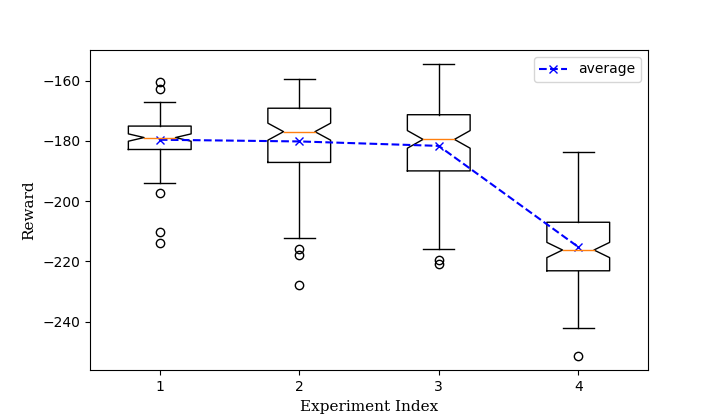
\includegraphics[scale=0.5]{graph/mcEvalBox.png}
  \caption{Evaluation notched box-plot for the MC environment, run for 1000 episodes.}
  \label{fig:mcEvalBox}
  \centering
    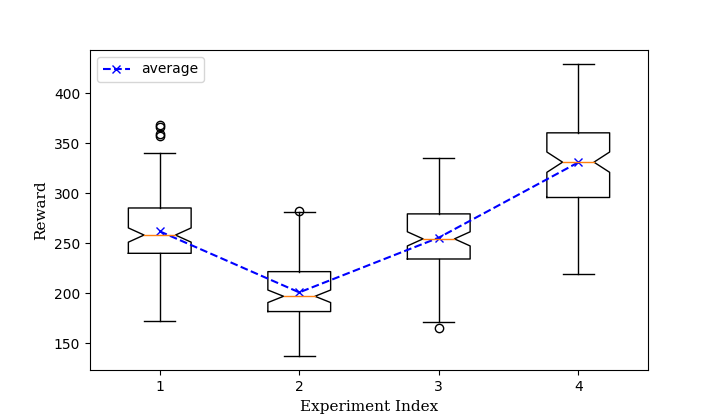
\includegraphics[scale=0.5]{graph/cpEvalBox.png}
  \caption{Evaluation notched box-plot for the CP environment, run for 1000 episodes.}
  \label{fig:cpEvalBox}
\end{figure}

Each of the agents are able to ‘solve’ their environments by the standards of OpenAi Gym, with the exception of on-policy DQL (4) for the MC environment. This is interesting as the same agent is the best performing on the CP environment by a large margin, whereas the inverse is true for MC. This is made yet stranger as the on-policy QL agent (2) is the worst performing on for CP with both off-policy agents (1, 3) performing at roughly the same level. Finally the other three agents (1-3) on MC have very similar average performance with the greatest concentration of results for off-policy QL (1). Whilst these results are interesting they do not pose any unexpected behaviour of the QL and DQL implementations.

The other results to be evaluated are those of the rewards distribution. If the results show that the distribution of the rewards are centered around the mean in a Gaussian distribution this is a normal distribution, representative of a real-values random sample of data. This evaluation will be conducted using histograms for each experiment and will be arranged in accordance to Table \ref{tab:indexHist} in Figures \ref{fig:mcEvalHist} and \ref{fig:cpEvalHist} for MC and CP respectively.

\begin{figure}[t]
  \centering
    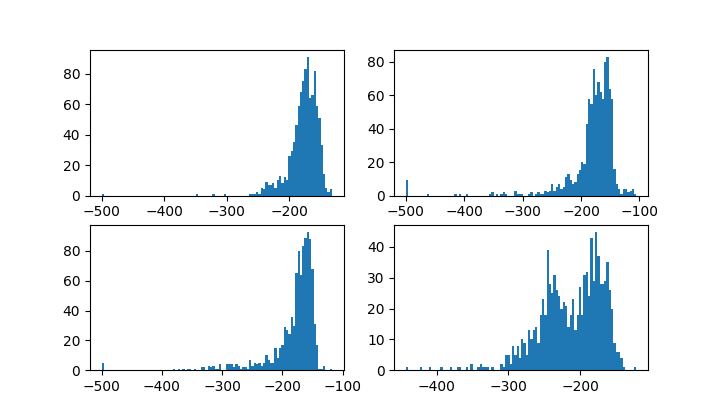
\includegraphics[scale=0.5]{graph/mcEvalHist.png}
  \caption{Evaluation histogram for the MC environment, run for 1000 episodes.}
  \label{fig:mcEvalHist}
  \centering
    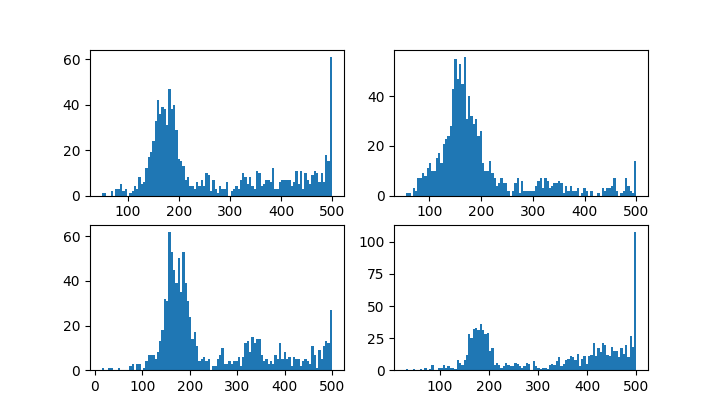
\includegraphics[scale=0.5]{graph/cpEvalHist.png}
  \caption{Evaluation histogram for the CP environment, run for 1000 episodes.}
  \label{fig:cpEvalHist}
\end{figure}

The bounds of the setup for the experiments being conducted prohibits a perfect normal distribution in that the possible reward gained is not continuous as the step limit is set at 500. However the distribution around the mean can still be checked to be suggestive of a normal distribution as a hallmark of an accurate sample of performance. If this is not the case then the performance is not stable, suggestive of an incorrectly functioning agent. Most of the agents do appear to have normal distributions from these histograms with two notable exceptions. These being the on-policy DQL agents (4) for both environments. The distribution of CP could potentially be explained by the step limit but that of the MC distribution clearly shows two peaks. Once again these results are interesting but are representative of the hypothesis posed and so do not invalidate the implementation. Extra focus will be placed on the on-policy DQL agent (4) in the following experimental analysis.
\subsection{Experiments}
\label{subsec:expExp}
As discussed previously, the experiments to be conducted are an analysis of the relative performances  of on-policy (Q-Learning) and off-policy (SARSA) control methods using the Q-Learning (QL) and Double Q-Learning (DQL) methods on the Mountain Car (MC) and Cart Pole (CP) control problems. These will be tested with a linear epsilon decay from 0.25, decaying to 0 at two thirds of the total episodes. The hyperparameters, alpha and gamma will be at a constant 0.5 and 0.995 respectively. The discretisation of the state observations will be 14 for MC and 6 for CP. The experimental setups described in \ref{tab:indexExp} will be run on both environments for 100, 250, 500 and 1000 episodes to examine how each setup’s performance varies at different training lengths.

Notched box-plots will be created from 100 averages of 10 individual runs to concentrate the plotted data and reduce the effect of anomalous results on the ranges of the plot axes. The reduction to 100 from 1000 results will produce less cluttered plots allowing for more precise interpretation. The averages will be recorded into a table and plotted as a line graph atop the box-plots to clearly show the variances between the experimental setups.

Histograms will be created from the total 1000 runs to show the distribution of results and compare against the results of the box-plots, checking that the sub-averaging of results is not dramatically distorting the data. The histograms will also aid in checking that the distributions of results are Gaussian, as another hallmark of reliable results. The averages of the 1000 runs will be recorded to be checked against the 100 averages of 10 runs to see that the disparity between them is not too large. These results will be organised into a table for readability.
\subsection{Results}
\label{subsec:expRes}
Overall the results for this experimental analysis could suggest that the hypothesis posed, discussing the best case performances for on-policy and off-policy control methods are related to the environmental factors. The results for CP show that on-policy methods do outperform off-policy methods in ‘action critical’ tasks and the same could be said for MC and off-policy methods. However the main observation that can me made from these results is that the DQL method has a high variance of performance than that of QL, this is shown best by the difference in distribution of reward between Experiments 1 and 3 in the histogram for 1000 episodes, Figure \ref{fig:cp4ResHist}. In this plot there is clearly a second distribution cluster for Experiment 3 but not for Experiment 1, this is in spite of their very similar averages for both the total average and sub-average. Additionally the distributions of results shown in the box-plot, Figure \ref{fig:cp4ResBox}, are very similar also. Whilst these results are suggestive of the hypothesis posed this is only at a surface level and appears to be greatest in the most severe cases, primarily that of Experiment 4 for both environments. Additionally the discrepancies between the average performances for the MC environment are rather serious, in the evaluation section above it was thought that the MC task had been solved by the first three agents and not the last but this is not the case. None of the agents solved the task when looking at the total average reward instead of the sub-averaged reward. The results listed in Table \ref{tab:results} once again support the hypothesis that on-policy methods perform better in action critical tasks for both the QL and DQL methods and the inverse is true for more general control problems in the case of off-policy control methods.

\begin{table*}[!ht]
  \centering
  \begin{tabular}{| c | c || c | c | c | c || c | c | c | c | }
    \hline
    \multicolumn{2}{|c||}{} & \multicolumn{8}{c|}{Training Episodes} \\ \cline{3-10}
  \multicolumn{2}{|c||}{Experiment Index} & \multicolumn{4}{c||}{Cart Pole $(+)$} & \multicolumn{4}{c|}{Mountain Car $(-)$} \\ \hline
  \multicolumn{2}{|c||}{} & 100 & 250 & 500 & 1000 & 100 & 250 & 500 & 1000 \\ \hline \hline
  \multirow{2}{*}{1} & Sub-average & 45.1 & 105.6 & 194.6 & 259.7 & 347.2 & 238.7 & 185.3 & 176.7 \\
                     & Average & 45.1 & 106.7 & 190.8 & 269.2 & 247.9 & 208.3 & 205.0 & 204.8 \\ \hline 
  \multirow{2}{*}{2} & Sub-average & 55.5 & 117.2 & 181.5 & 205.1 & 391.4 & 284.6 & 224.9 & 185.7 \\
                     & Average & 58.1 & 114.8 & 160.1 & 199.7 & 299.0 & 240.6 & 213.7 & 214.1 \\ \hline 
  \multirow{2}{*}{3} & Sub-average & 85.8 & 157.5 & 166.0 & 254.6 & 381.4 & 271.1 & 228.0 & 178.9 \\
                     & Average & 87.6 & 151.1 & 177.8 & 252.7 & 307.9 & 219.8 & 207.9 & 206.8 \\ \hline 
  \multirow{2}{*}{4} & Sub-average & 119.3 & 177.4 & 232.8 & 334.1 & 399.4 & 298.7 & 218.2 & 213.4 \\
                     & Average & 117.5 & 177.6 & 239.6 & 324.5 & 299.0 & 254.2 & 255.8 & 254.2 \\ \hline 
  \end{tabular}
  \caption{Averages for each experiment}
  \label{tab:results}
\end{table*}

\begin{figure}[p]
  \centering
  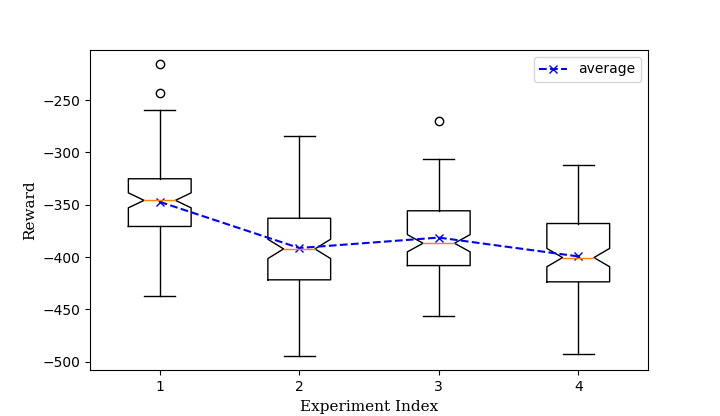
\includegraphics[scale=0.45]{graph/mc1ResBox.png}
  \caption{Notched box-plot for the MC environment, run for 100 episodes.}
  \label{fig:mc1ResBox}
  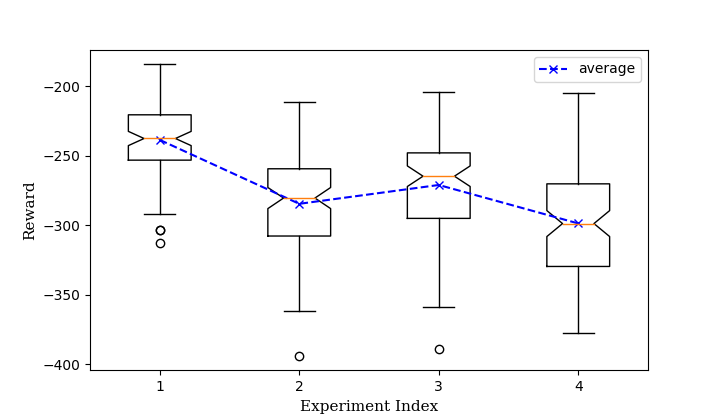
\includegraphics[scale=0.45]{graph/mc2ResBox.png}
  \caption{Notched box-plot for the MC environment, run for 250 episodes.}
  \label{fig:mc2ResBox}
  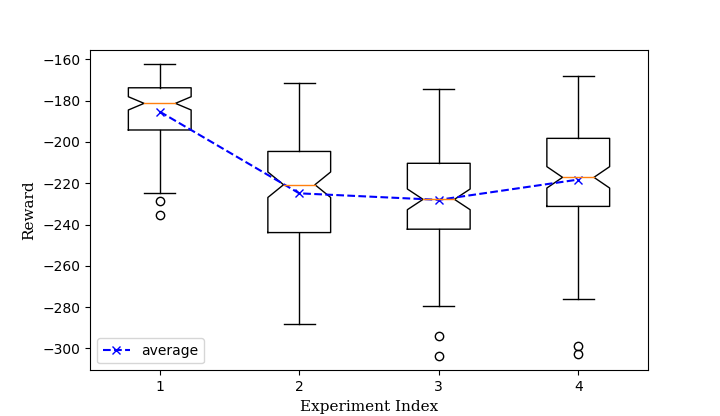
\includegraphics[scale=0.45]{graph/mc3ResBox.png}
  \caption{Notched box-plot for the MC environment, run for 500 episodes.}
  \label{fig:mc3ResBox}
  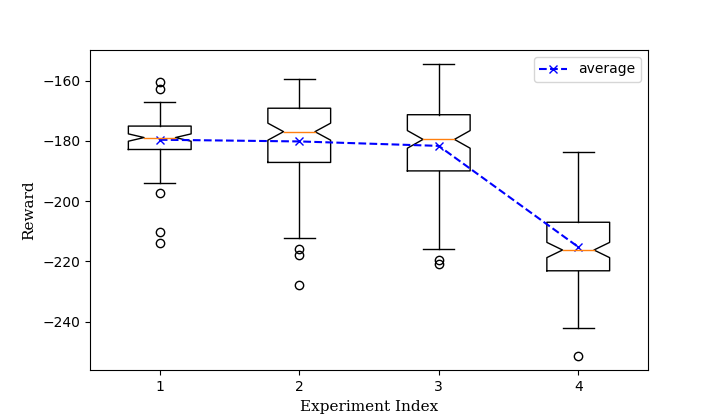
\includegraphics[scale=0.45]{graph/mcEvalBox.png}
  \caption{Notched box-plot for the MC environment, run for 1000 episodes.}
  \label{fig:mc4ResBox}
\end{figure}

\begin{figure}[p]
  \centering
  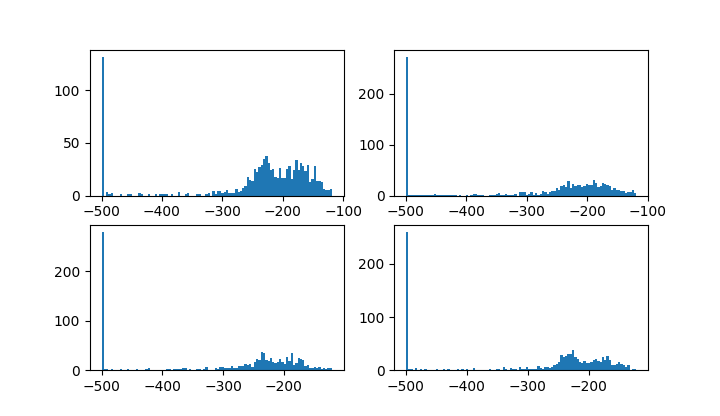
\includegraphics[scale=0.45]{graph/mc1ResHist.png}
  \caption{Histogram for the MC environment, run for 100 episodes.}
  \label{fig:mc1ResHist}
  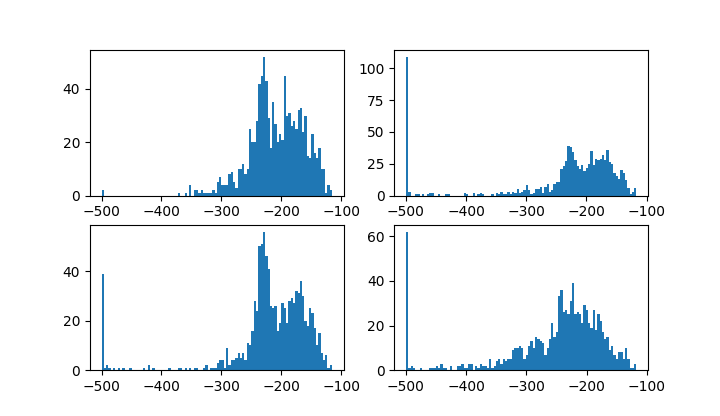
\includegraphics[scale=0.45]{graph/mc2ResHist.png}
  \caption{Histogram for the MC environment, run for 250 episodes.}
  \label{fig:mc2ResHist}
  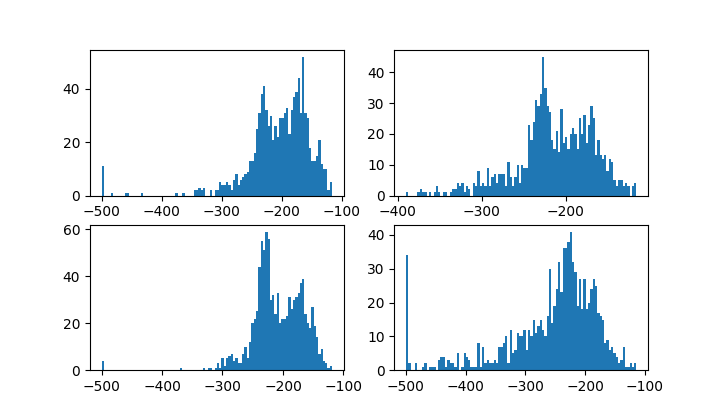
\includegraphics[scale=0.45]{graph/mc3ResHist.png}
  \caption{Histogram for the MC environment, run for 500 episodes.}
  \label{fig:mc3ResHist}
  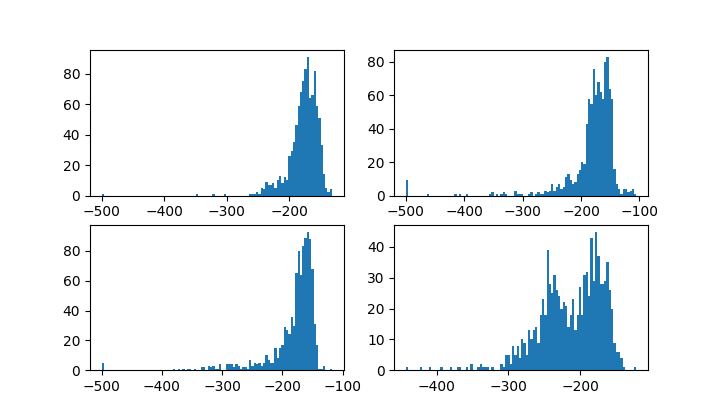
\includegraphics[scale=0.45]{graph/mcEvalHist.png}
  \caption{Histogram for the MC environment, run for 1000 episodes.}
  \label{fig:mc4ResHist}
\end{figure}

\begin{figure}[p]
  \centering
  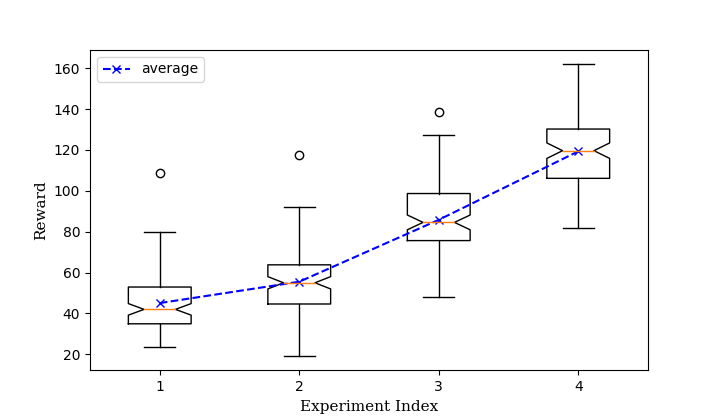
\includegraphics[scale=0.45]{graph/cp1ResBox.png}
  \caption{Notched box-plot for the CP environment, run for 100 episodes.}
  \label{fig:cp1ResBox}
  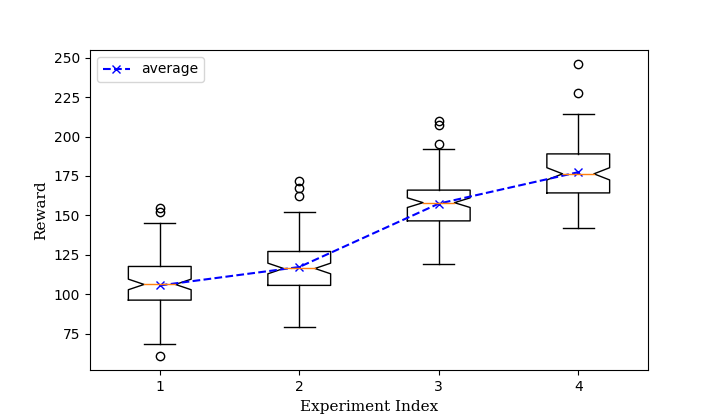
\includegraphics[scale=0.45]{graph/cp2ResBox.png}
  \caption{Notched box-plot for the CP environment, run for 250 episodes.}
  \label{fig:cp2ResBox}
  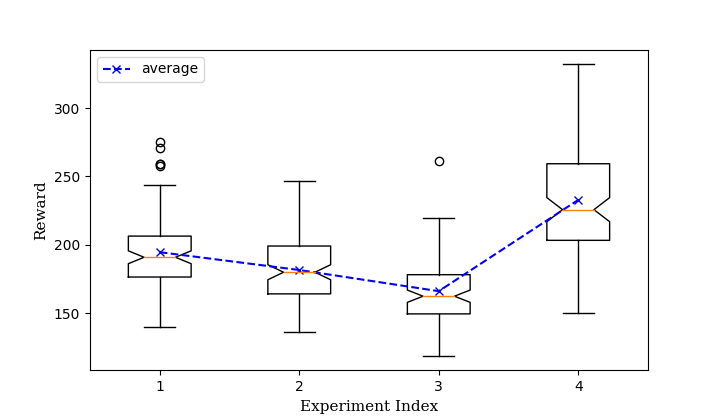
\includegraphics[scale=0.45]{graph/cp3ResBox.png}
  \caption{Notched box-plot for the CP environment, run for 500 episodes.}
  \label{fig:cp3ResBox}
  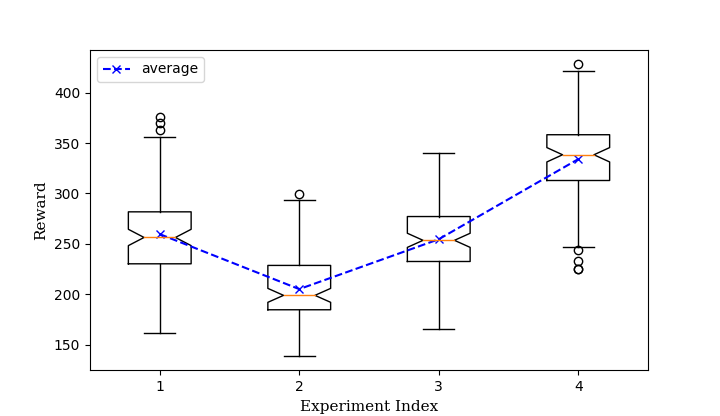
\includegraphics[scale=0.45]{graph/cp4ResBox.png}
  \caption{Notched box-plot for the CP environment, run for 1000 episodes.}
  \label{fig:cp4ResBox}
\end{figure}

\begin{figure}[p]
  \centering
  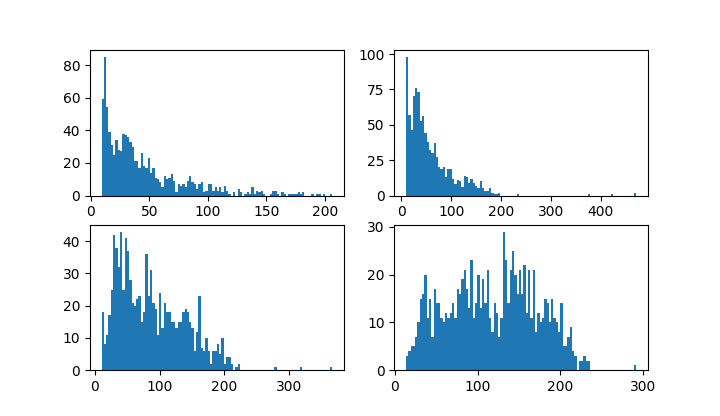
\includegraphics[scale=0.45]{graph/cp1ResHist.png}
  \caption{Histogram for the CP environment, run for 100 episodes.}
  \label{fig:cp1ResHist}
  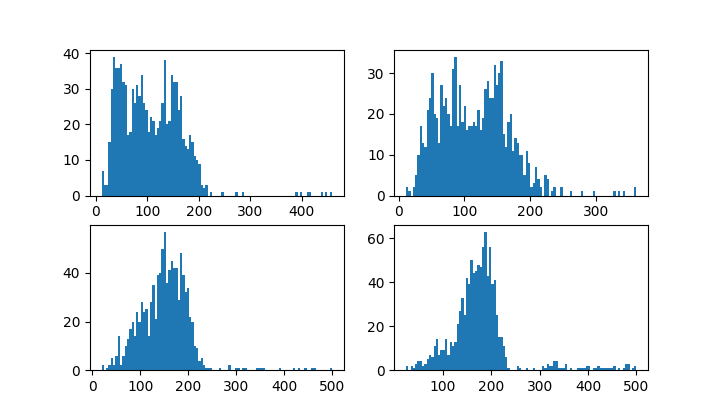
\includegraphics[scale=0.45]{graph/cp2ResHist.png}
  \caption{Histogram for the CP environment, run for 250 episodes.}
  \label{fig:cp2ResHist}
  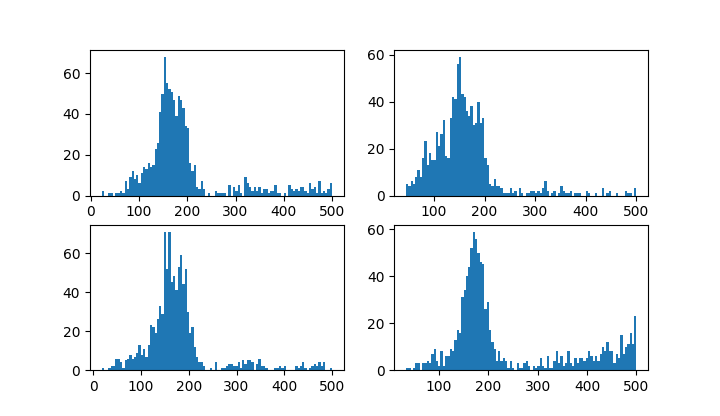
\includegraphics[scale=0.45]{graph/cp3ResHist.png}
  \caption{Histogram for the CP environment, run for 500 episodes.}
  \label{fig:cp3ResHist}
  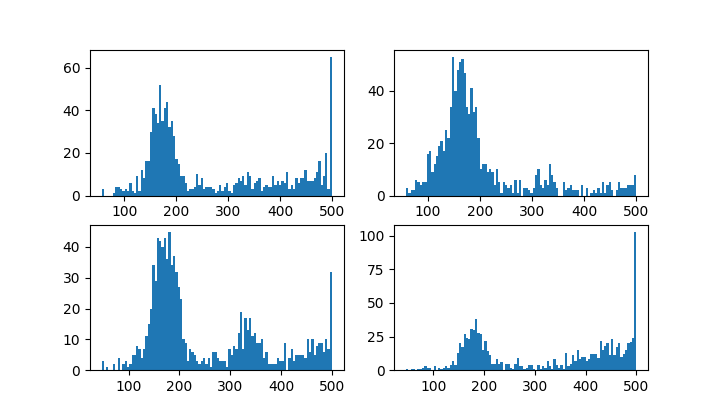
\includegraphics[scale=0.45]{graph/cp4ResHist.png}
  \caption{Histogram for the CP environment, run for 1000 episodes.}
  \label{fig:cp4ResHist}
\end{figure}

\section{Discussions and Reflective Analysis}
\label{sec:discussions}
My view of the project as a whole is very positive, I learned a lot about RL and enjoyed the development of the artefact. However I feel as though the design of my methodology was naive and my implementation of it in certain processes was poor. Overall I am pleased with this project and feel as though I achieved what I set out to do.

In spite of the personal circumstances surrounding this project\footnote{See Appendix \ref{apx:personalDifficulties} for more detail} and the many delays in its completion, I am very happy with the outcome and hope to continue to develop upon this project in the future. In particular I am happy with the project management skills I have developed as well as my new appreciation of source control which I feel will be invaluable to me in the future.

One particular aspect I am very pleased with about this project is how it has expanded my experience with the scientific computing tools used. I had certainly used Python and Numpy previously to good effect but it seems as though their compatibility with TD problems is incredible. Aside from plotting with Matplotlib and use of OpenAi Gym for environments, the only external Python dependency used is Numpy and I am amazed by its capabilities. Most other projects I have undertaken in this area of study have required numerous libraries and a lot of reading of documentation to effectively use. The benefit of using a few very simple tools to develop such a complex system meant that my development efforts were incredibly focused. Where usually I would spend a lot of time reading various articles online to eventually find what documentation I should be reading to complete a specific task, the focused nature of the project allowed rapid development in all areas. When I ran into something I didn’t know how to do I could almost instantly find the Numpy or Python native functions which should be used. The benefit this was to the entire software development process is very hard to convey and measure but I hope that this project can serve as a springboard. So that other people like me with rudimentary scientific computing skills to engage with this field. As the barrier to entry is not terribly high, the only difficulty I encountered was that there was little in the academic literature explaining how these rather abstract systems can be implemented in a programmatic fashion. This experience of \textit{getting my teeth} into the simplicity of TD problems, has encouraged me to expand this project beyond this dissertation in the future, to give a guideline of how to use RL in practice. Sadly this is a difficult thing to academically justify and so there is little room for expansion in this dissertation, although I have tried where possible.
\subsection{Academic Study}
\label{subsec:dissStud}
I was pleased overall with the breadth of academic literature I was able to study in support of this project, however I have always read very slowly and so I feel as though the time spent studying and researching was at times prohibitive to the project as a whole. Additionally, when I felt as though I had more questions to research later on in the project, I was always able to find literature that would have been useful to have studied earlier on in the process. I think that in many ways the methods used to find relevant literature were particularly weak and left a level of doubt in my mind that I was perhaps not grasping the entire picture. The literature surveys I read are the only examples of concrete academic literature study methodologies \parencite{Kober13, Busoniu08, Kaelbling96, Wirth17} I could find discussed in detail. In many ways I can see why as in \textcite{Ahmad17} these methods of systematic literature surveys seem prohibitively ‘long-winded’ and I feel as though they would each be overboard for a project such as this. But perhaps this is par for the course in academic study and the feeling of always finding more was simply my advancing understanding of the subject. Indeed I feel as though more thought in this area before beginning the implementation would have been highly beneficial.
\subsection{Development}
\label{subsec:dissDevel}
If more time had been available it would have been useful to do an iteration upon the study once the results had been analysed. With the results gathered there was certainly a difference observed but the information needed to understand what may be causing this discrepancy was lacking. I would have liked to add plots for showing the action selections over time to understand how the agents interacted with the environments.
\subsection{Evaluation}
\label{subsec:dissEval}
Whilst the evaluation of the developed agents achieved the aims of the objectives set out in Section \ref{subsec:intAimAndObj}, they would appear to me to not be rigorous enough to directly support the hypotheses posed. Additionally, the assessment of this literature to investigate why the disparity between on-policy and off-policy could only find suggestions towards which applications would best suit the two control methods and little discussion as to the mechanics behind the difference. It would appear from the surrounding research into more advanced TD learning methods that perhaps the two work best when combined \cite{Wang13, Zhi-Xiong18} to revise the learned policy into a more robust policy retroactively using SARSA after QL has been used to learn the initial policy. This application has been used in both \textcite{Wang13} for traditional RL and by \textcite{Zhi-Xiong18} for deep RL with experience replay.

There is indeed a difference between on-policy and off-policy control methods. However, I feel as though my experimental analysis did not go far enough to prove the hypotheses posed in Section \ref{subsec:intHypothesis} as to why this might be the case. If I were to perform this analysis again I would gather far more information from the training process, such as actions taken, and represent how the Q-values change with each iteration. Had computing resources not been limited I would also have liked to use longer training periods and higher max step counts, however these represented a large addition to the computing time required.

Finally I should have reached out to my supervisors for help in deciding which  statistical methods to use for the analysis. Whilst I feel as though the majority of the direct empirical data was gathered, there was not enough surrounding information to perform the analysis I had intended to. Although I do feel as though there is a good basis from which future research could expand this analysis to a more complete investigation.
\subsection{Time Management}
\label{subsec:dissTime}
One of the particularly troublesome areas in this project was time management, in particular the hardware bottleneck discussed in Section \ref{subsubsec:desReqReq} led to a constant need to be running the agents. To get results for tuning as well as results suggestive of the overall performance of the agents took a very long time due to the computational limits of Q-Learning. This led to a habit of keeping things running at all times, trying to squeeze as much information as possible from the agents. However, this habit caused multiple useless runs of agents due to syntactical mistakes and otherwise misguided experiments. A Kanban board implemented alongside the development stage, to manage testing, would have saved an inordinate amount of time as each test would be planned out. Even the nature of Kanban boards would suit this use-case as since there is a hard limit on the number of processes that can be run at one time; This being 8, the number of cores in my CPU. This is perhaps the largest missed opportunity for implementation of methodological structure in this project. The work-in-progress column could have pulled from a pool of planned experiments with a hard limit of 8. These then could pass into the review column where the results are recorded and indexed and finally moved to the completed section. This could well have eliminated most of the waste from the experimentation phase and in turn made the analysis of the agents much more effective.

Beyond this missed opportunity for methodological implementation was the time wasted by my distraction from the task I was working on to constantly busy myself over the computational process was immeasurable. Although a tool for integration into Trello for example would allow this process to be augmented. Instead of manually running, each experiment a Kanban board could be used as described above, pulling new tasks into the work-in-progress and moving on to another once it is completed automatically using a client and Trello extension. These completed experiments could automatically record the results and plots, storing on the trello board within the relevant card for review at a later stage. This is a strong example for future development and research which would be very easy to integrate into the developed artefact as a testing ground.

An aspect of this RL project when compared to previous machine learning projects personally undertaken, is how the developmental criteria grows as more is learned about the problem domain. Each target set for completion time was pushed back by an exponentially growing list of potential optimisations and issues to be developed. This particularly hampered the evaluation stage as each time the results gathered were analysed it led to more questions about the way the agents operated. As an example, the bug discussed in Section \ref{subsec:dissDevel}, found in the very late stages of evaluation that a piece of legacy code had remained in the DQL class but not the QL class. This was a simple modification to the calculation of the discrete state from the continuous state, once addressed it became obvious that this could be the cause of the discrepancy between odd and even discretisation factors which had been tested and used in what was supposed to be in the final analysis of the agents. Potentially invalidating the results, as discussed previously the computational requirements for comprehensive testing are high and so the potential effect of this bug upon the time taken for this analysis was huge. But additionally this opens up new questions about how this bug had not been catastrophic to the computation of the agent as it would cause indexing errors which was the original reason for the modification being made. This is a strong example of how code review should have been used in such a computationally complex problem to catch small \textit{five character} differences like this before they can have an impact on the results gathered. It would be hard to balance the process as a whole however, since realisations like this were only possible once a lot of experience with RL had been gained. Indeed I feel as though the only way to avoid problems like this would be to not carry legacy code forward, which should perhaps have been a key feature of the software development methodology. For example the development stages could have been discretised with experience informing the development of the next stage from scratch instead of the code refactoring method used.

\subsection{Mental Blocks}
One aspect of understanding in this project which eluded me until I came to write how it works in this report, is how the reward function ‘back-propagates’ to cause the temporal optimisation which TD learning functions upon. I had implemented it and even observed it happening, but had never grasped that it was the process of assessing the next action to update the current action values which causes this style of learning in TD models. Even now I am amazed how I completed this project without understanding this fundamental concept. Despite all the research done on the subject and relatively firm grasp on all of the surrounding TD concepts; I never realised the fundamental core of how TD operates. I would put the blame on the literature I have read, but I’m certain that cannot be the case, perhaps it was assumed as an obvious result of TD models. But I can only speculate, I feel as though if I had taken the time to ponder the theory I was researching and implementing I may have grasped this sooner. But as it is I cannot believe how much of a fool I was. If I were to do this project again with more time to stop and think...
\section{Conclusion}
\label{sec:conclusion}
The differences between on-policy and off-policy control methods are certainly present, as demonstrated in this study, which appears to be largely overlooked in the literature. This is confusing as QL is so foundational to the myriad of methods which followed on from its definition in \textcite{Watkins89}. Whereas the very similar method described in \textcite{Rummery94} has seen little attention aside from incorporations into existing QL methods. This is very strange and the little discussion found comparing the two comes to little conclusion as to their relative performances. The only substantive discussion on this is in \textcite{Corozza15} which is so tightly focused on financial trading that very few of its findings are directly related to the control problems studied in this project.

The comparative analysis done on the two control policies in this project was inconclusive and could only be said to suggest that the hypothesis posed may be valid. But as it stands there is very little to substantiate that on. There is evidence for a discrepancy between the control methods when applied to the MC and CP control problems but that is all. More research is certainly needed on this subject and a more substantive analysis would be required to explore the differences encountered in this study.

\addcontentsline{toc}{section}{References}
\setlength\bibitemsep{1.7\itemsep plus 1pt minus 1pt}
\printbibliography

\addcontentsline{toc}{section}{Acknowledgements}
\section*{Acknowledgements}
I dedicate this dissertation to my family and friends, without their support I would never have had the strength to continue this project.

I must commend the lengths to which my peers helped me refine the writing in this document. My lexical abilities have always been a large weak point and this report would have been so much worse for it, without the help of my proof reading team, in particular my fiends Luci Goldup, Leo Kyle, Cat Flynn, Nate James and my sister Catrin Ody. Thank you.

Particular thanks must be extended to Daniel Holden who helped in explaining the statistical notation foundational to this project.

The recommendation of my project supervisor Stefanos Kollias to dial back the ambition of this project as it was initially proposed was needed and I think him for it.

A final thank you to my \emph{'rubber ducks'}, Nate James and Cat Flynn, who allowed me to discuss issues in this project with them at length; which was invaluable in my conception of these issues and subsequent solution.

\begin{appendices}

\section{Extended Discussion}
\subsection{Taxi Environment}
\label{apx:taxi}
The first stage of the development was to get a functional QL implementation, to this end, a simple ‘toy text’ environment was chosen from the OpenAI Gym library (\url{https://gym.openai.com/envs/#toy_text}). This was ‘Taxi-v2’ (\url{https://gym.openai.com/envs/Taxi-v2/}) which was chosen for its simplicity. Taxi is a gridworld-like environment with $25$ $(5\times5)$ tiles and $4$ locations. The aim is to pick-up the passenger at their location and transport them to their destination. The reward function gives $+20$ whenever a passenger is successfully delivered and $-1$ for each step. A reward of $-10$ is given for each illegal pickup or dropoff action made. This at first glance seems like a complex problem, however there is no dynamic behaviour, this means that the problem is random yet deterministic in nature. In practice this makes it very fast to solve but at the same time complex enough to test the capabilities of an RL solution. Additionally, the environment can be rendered in text alone and so makes direct observation of the agent behaviour both efficient and clear.

\subsection{Trials and Tribulations}\label{apx:personalDifficulties}
I have long suffered from high-functioning depression, but had considered it \textit{'beaten'} around the time I came to university in 2015. If only I had known that my first breath of normalcy was just that, and not the sustainable happiness I had long sought after. Over my time at university I regressed back into old ways and habits until the end of my Masters, in the summer of 2019 I reached a breaking point. In a panic I threw caution to the wind and scrapped this very project I had been working on for submission in August, in a desperate attempt to salvage my mental state. After pulling myself back together I realised that I really did want to continue my academic study, and thanks to the wonderful support of the university staff I was able to continue this research project.

In particular I would like to thank Victoria Bryant and Bashir Al-Diri for being so understanding and accommodating of me when I was most vulnerable.

As of writing this a few months down the line at the turn of 2020 I am amazed by how far I have come already, I know I will beat it this time.

Thank you,

Tom

\section{Source Code}
\label{apx:sourceCode}
\subsection{Single Q-Learning Class}
\label{apx:sinKew}
sinKew.py
\pythonexternal{code/sinKew.py}

\subsection{Double Q-Learning Class}
\label{apx:dblKew}
dblKew.py
\pythonexternal{code/dblKew.py}

\subsection{Experiment Harness}
\label{apx:exp}
exp.py
\pythonexternal{code/exp.py}

\subsection{Run script}
\label{apx:do}
do.py
\pythonexternal{code/do.py}

\subsection{Cart Pole Comparison}
\label{apx:cp}
cp.py
\pythonexternal{code/cp.py}

\subsection{Mountain Car Comparison}
\label{apx:mc}
mc.py
\pythonexternal{code/mc.py}

\onecolumn
\section{Full Size Figures}
\label{apx:figures}
\subsection{Cart Pole Evaluation}
\begin{figure}[!h]
  \centering
  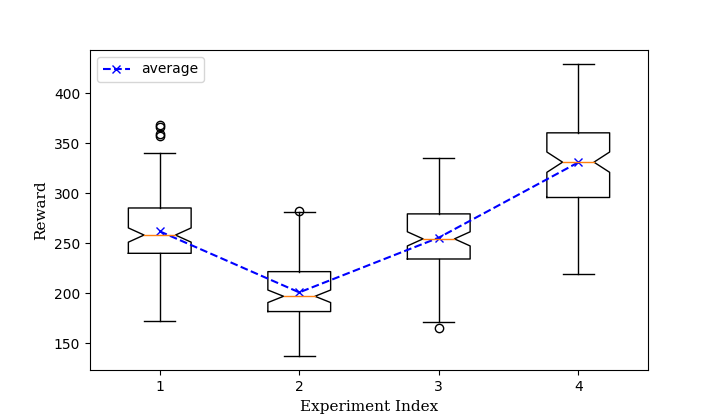
\includegraphics[scale=1]{graph/cpEvalBox.png}
  \caption{Evaluation notched box-plot for the CP environment, run for 1000 episodes.}
  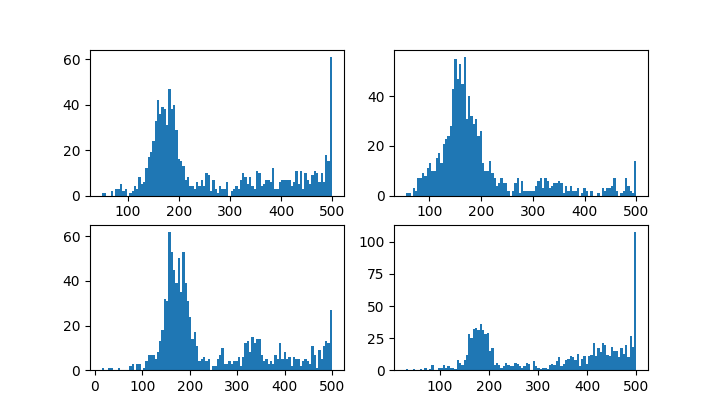
\includegraphics[scale=1]{graph/cpEvalHist.png}
  \caption{Evaluation histogram for the CP environment, run for 1000 episodes.}
\end{figure}
\pagebreak

\subsection{Mountain Car Evaluation}
\begin{figure}[!h]
  \centering
  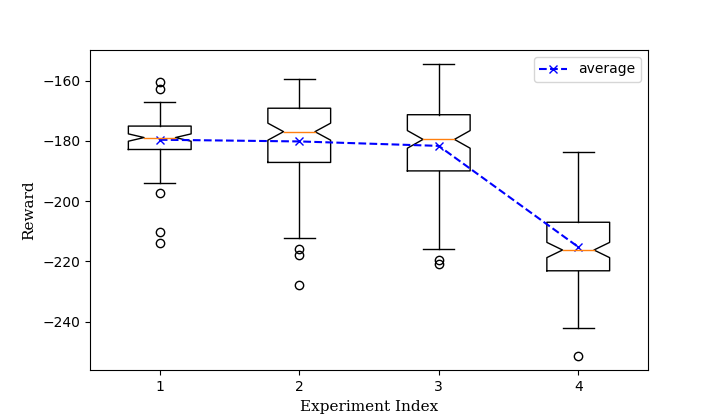
\includegraphics[scale=1]{graph/mcEvalBox.png}
  \caption{Evaluation notched box-plot for the MC environment, run for 1000 episodes.}
  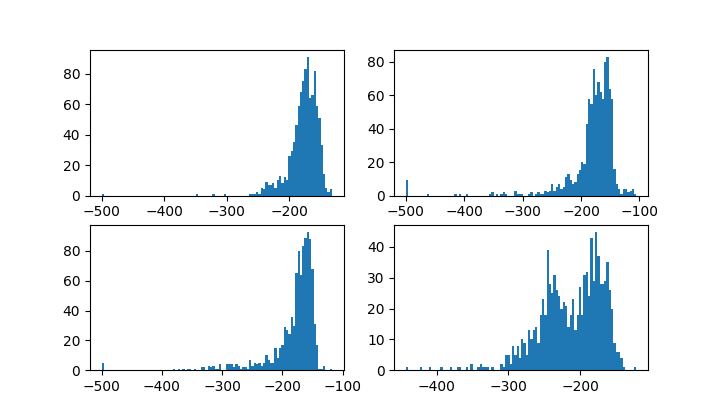
\includegraphics[scale=1]{graph/mcEvalHist.png}
  \caption{Evaluation histogram for the MC environment, run for 1000 episodes.}
\end{figure}
\pagebreak

\subsection{Cart Pole Results}

\begin{figure}[!h]
  \centering
  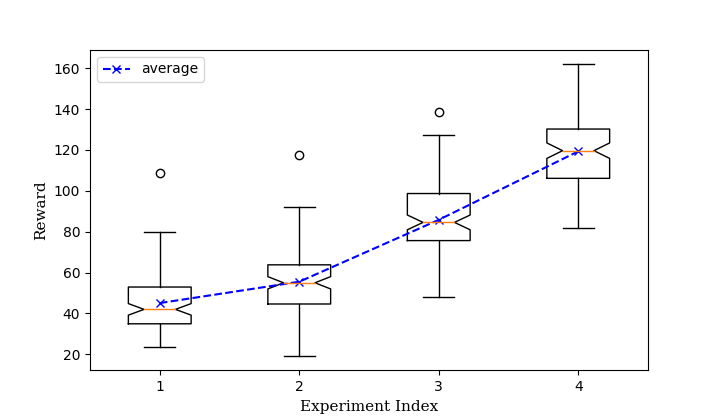
\includegraphics[scale=1]{graph/cp1ResBox.png}
  \caption{Notched box-plot for the CP environment, run for 100 episodes.}
  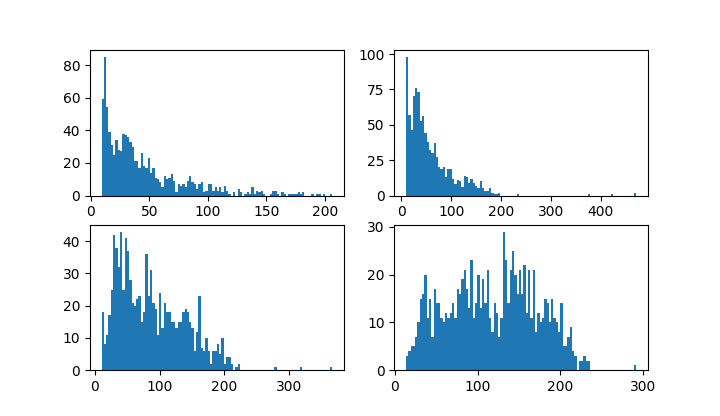
\includegraphics[scale=1]{graph/cp1ResHist.png}
  \caption{Histogram for the CP environment, run for 100 episodes.}
\end{figure}

\pagebreak

\begin{figure}[!h]
  \centering
  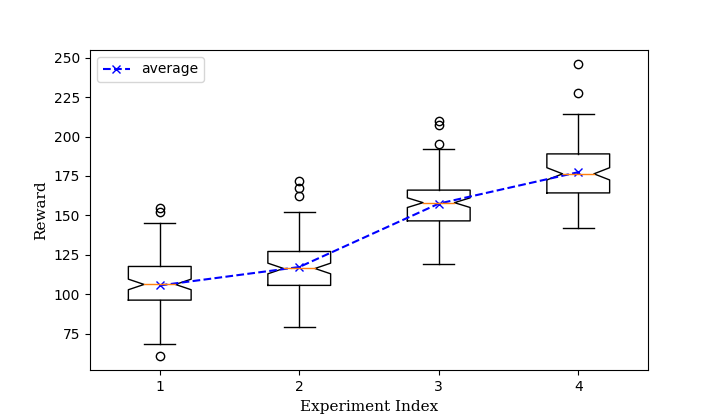
\includegraphics[scale=1]{graph/cp2ResBox.png}
  \caption{Notched box-plot for the CP environment, run for 250 episodes.}
  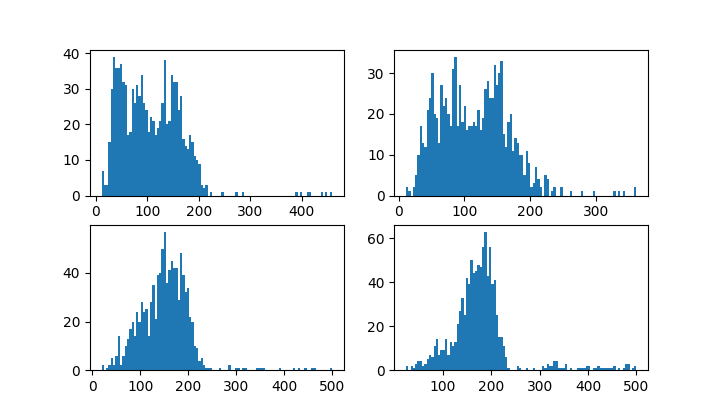
\includegraphics[scale=1]{graph/cp2ResHist.png}
  \caption{Histogram for the CP environment, run for 250 episodes.}
\end{figure}

\pagebreak

\begin{figure}[!h]
  \centering
  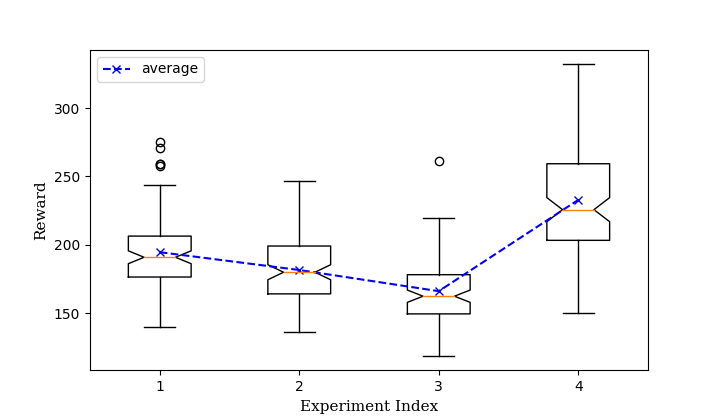
\includegraphics[scale=1]{graph/cp3ResBox.png}
  \caption{Notched box-plot for the CP environment, run for 500 episodes.}
  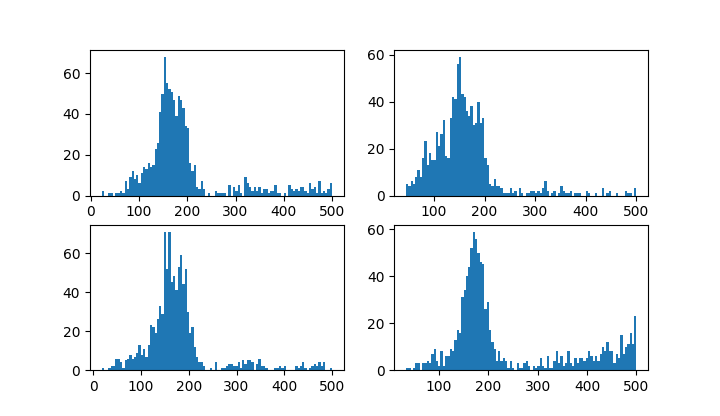
\includegraphics[scale=1]{graph/cp3ResHist.png}
  \caption{Histogram for the CP environment, run for 500 episodes.}
\end{figure}
\pagebreak

\begin{figure}[!h]
  \centering
  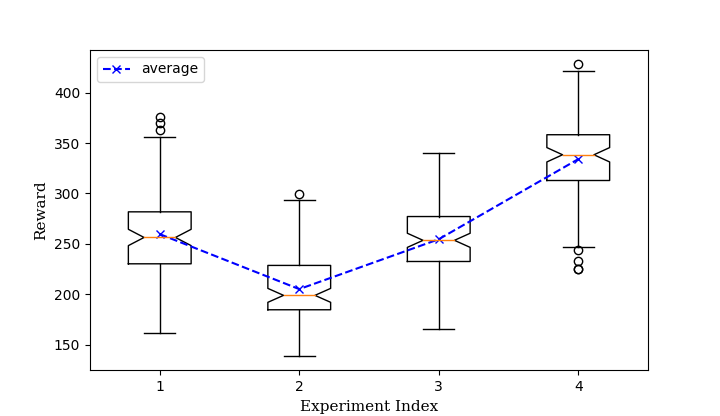
\includegraphics[scale=1]{graph/cp4ResBox.png}
  \caption{Notched box-plot for the CP environment, run for 1000 episodes.}
  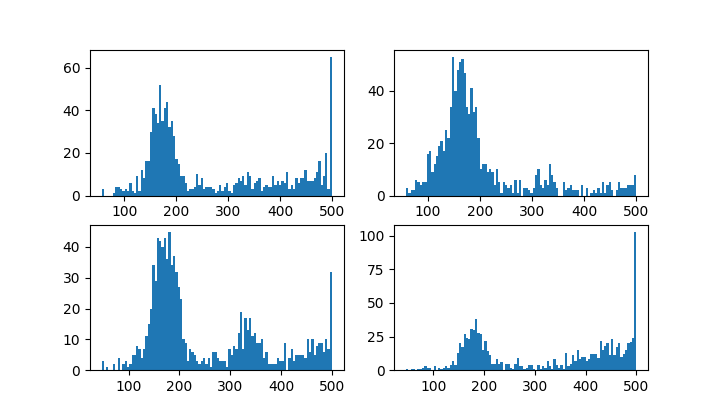
\includegraphics[scale=1]{graph/cp4ResHist.png}
  \caption{Histogram for the CP environment, run for 1000 episodes.}
\end{figure}

\pagebreak

\subsection{Mountain Car Results}

\begin{figure}[!h]
  \centering
  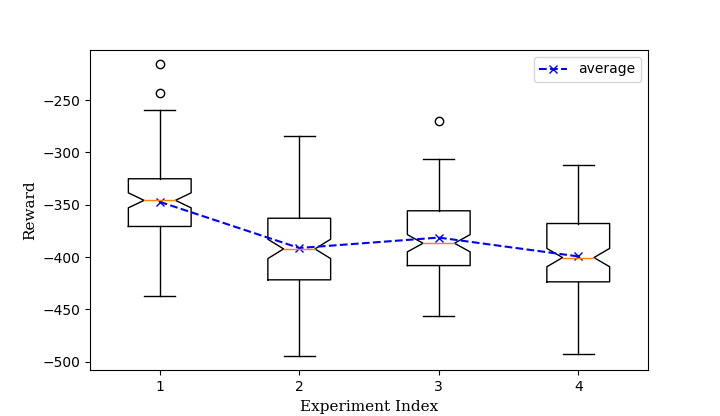
\includegraphics[scale=1]{graph/mc1ResBox.png}
  \caption{Notched box-plot for the MC environment, run for 100 episodes.}
  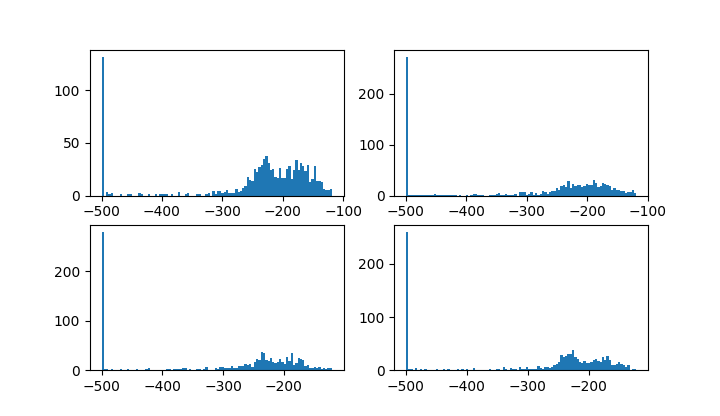
\includegraphics[scale=1]{graph/mc1ResHist.png}
  \caption{Histogram for the MC environment, run for 100 episodes.}
\end{figure}

\pagebreak

\begin{figure}[!h]
  \centering
  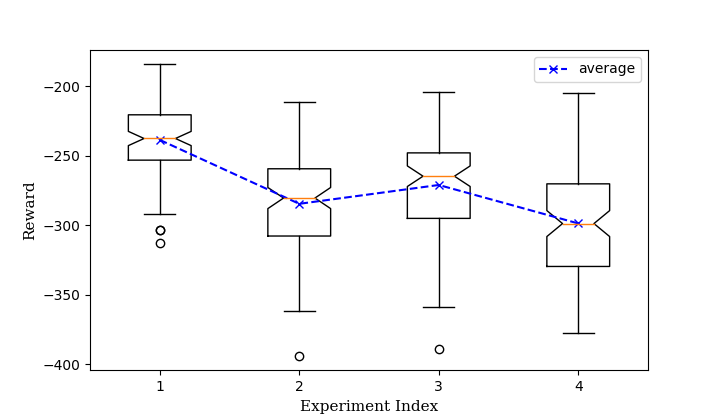
\includegraphics[scale=1]{graph/mc2ResBox.png}
  \caption{Notched box-plot for the MC environment, run for 250 episodes.}
  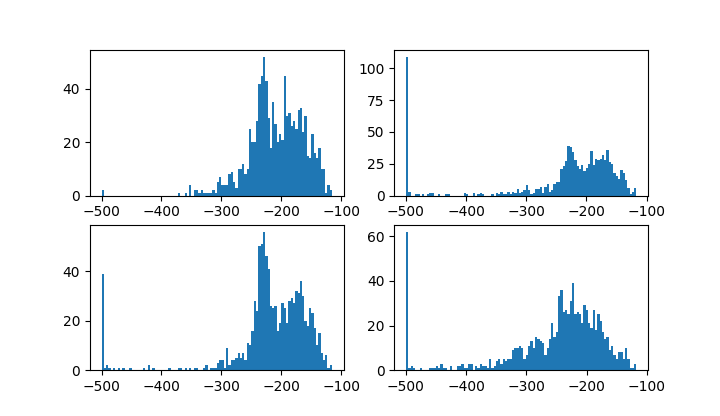
\includegraphics[scale=1]{graph/mc2ResHist.png}
  \caption{Histogram for the MC environment, run for 250 episodes.}
\end{figure}

\pagebreak

\begin{figure}[!h]
  \centering
  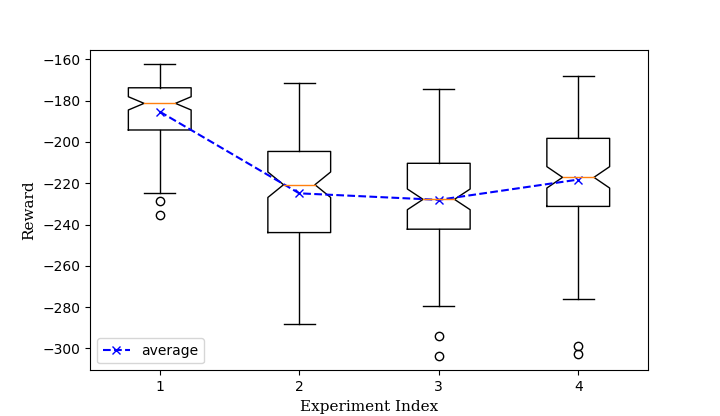
\includegraphics[scale=1]{graph/mc3ResBox.png}
  \caption{Notched box-plot for the MC environment, run for 500 episodes.}
  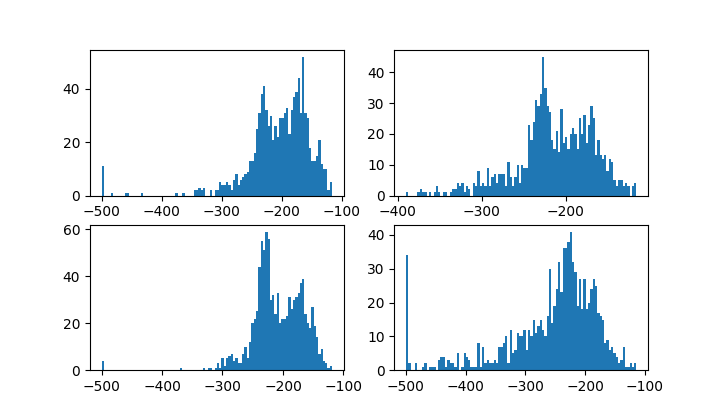
\includegraphics[scale=1]{graph/mc3ResHist.png}
  \caption{Histogram for the MC environment, run for 500 episodes.}
\end{figure}

\pagebreak

\begin{figure}[!h]
  \centering
  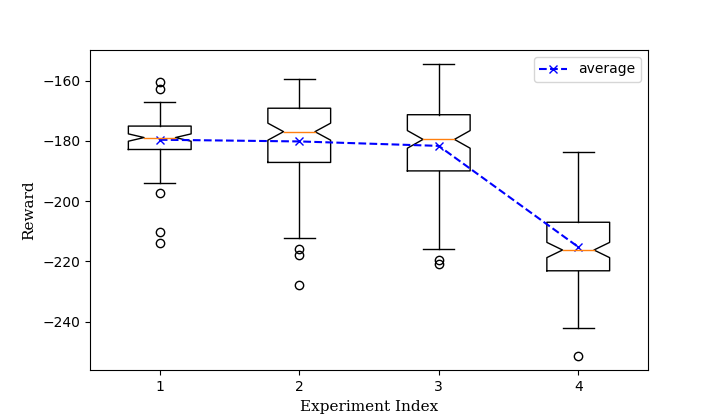
\includegraphics[scale=1]{graph/mcEvalBox.png}
  \caption{Notched box-plot for the MC environment, run for 1000 episodes.}
  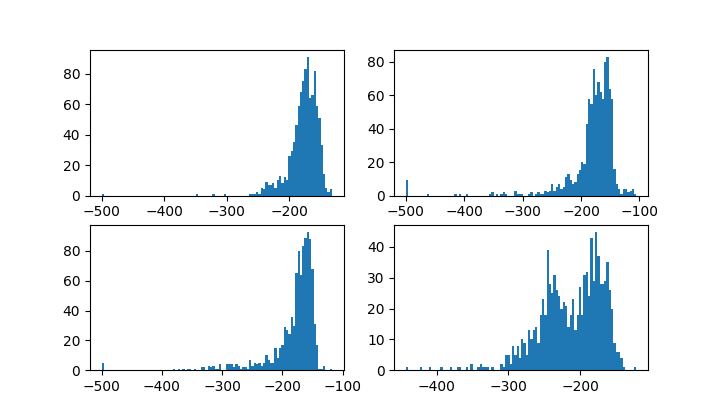
\includegraphics[scale=1]{graph/mcEvalHist.png}
  \caption{Histogram for the MC environment, run for 1000 episodes.}
\end{figure}

\pagebreak

\end{appendices}

\end{document}
